% Options for packages loaded elsewhere
\PassOptionsToPackage{unicode}{hyperref}
\PassOptionsToPackage{hyphens}{url}
%
\documentclass[
]{article}
\usepackage{amsmath,amssymb}
\usepackage{iftex}
\ifPDFTeX
  \usepackage[T1]{fontenc}
  \usepackage[utf8]{inputenc}
  \usepackage{textcomp} % provide euro and other symbols
\else % if luatex or xetex
  \usepackage{unicode-math} % this also loads fontspec
  \defaultfontfeatures{Scale=MatchLowercase}
  \defaultfontfeatures[\rmfamily]{Ligatures=TeX,Scale=1}
\fi
\usepackage{lmodern}
\ifPDFTeX\else
  % xetex/luatex font selection
\fi
% Use upquote if available, for straight quotes in verbatim environments
\IfFileExists{upquote.sty}{\usepackage{upquote}}{}
\IfFileExists{microtype.sty}{% use microtype if available
  \usepackage[]{microtype}
  \UseMicrotypeSet[protrusion]{basicmath} % disable protrusion for tt fonts
}{}
\makeatletter
\@ifundefined{KOMAClassName}{% if non-KOMA class
  \IfFileExists{parskip.sty}{%
    \usepackage{parskip}
  }{% else
    \setlength{\parindent}{0pt}
    \setlength{\parskip}{6pt plus 2pt minus 1pt}}
}{% if KOMA class
  \KOMAoptions{parskip=half}}
\makeatother
\usepackage{xcolor}
\usepackage[margin=1in]{geometry}
\usepackage{graphicx}
\makeatletter
\def\maxwidth{\ifdim\Gin@nat@width>\linewidth\linewidth\else\Gin@nat@width\fi}
\def\maxheight{\ifdim\Gin@nat@height>\textheight\textheight\else\Gin@nat@height\fi}
\makeatother
% Scale images if necessary, so that they will not overflow the page
% margins by default, and it is still possible to overwrite the defaults
% using explicit options in \includegraphics[width, height, ...]{}
\setkeys{Gin}{width=\maxwidth,height=\maxheight,keepaspectratio}
% Set default figure placement to htbp
\makeatletter
\def\fps@figure{htbp}
\makeatother
\setlength{\emergencystretch}{3em} % prevent overfull lines
\providecommand{\tightlist}{%
  \setlength{\itemsep}{0pt}\setlength{\parskip}{0pt}}
\setcounter{secnumdepth}{5}
\usepackage{booktabs}
\usepackage{longtable}
\usepackage{array}
\usepackage{multirow}
\usepackage{wrapfig}
\usepackage{float}
\usepackage{colortbl}
\usepackage{pdflscape}
\usepackage{tabu}
\usepackage{threeparttable}
\usepackage{threeparttablex}
\usepackage[normalem]{ulem}
\usepackage{makecell}
\usepackage{xcolor}
\ifLuaTeX
  \usepackage{selnolig}  % disable illegal ligatures
\fi
\usepackage{bookmark}
\IfFileExists{xurl.sty}{\usepackage{xurl}}{} % add URL line breaks if available
\urlstyle{same}
\hypersetup{
  pdftitle={Etude statistique},
  hidelinks,
  pdfcreator={LaTeX via pandoc}}

\title{Etude statistique}
\author{}
\date{\vspace{-2.5em}2025-03-10}

\begin{document}
\maketitle

{
\setcounter{tocdepth}{2}
\tableofcontents
}
\section{Introduction}\label{introduction}

Cette étude statistique a pour but d'analyser les comportements et
ressentis des joueurs de football avant un match. Nous explorons
notamment la relation entre l'expérience et l'anxiété, ainsi que les
difficultés rencontrées. L'étude repose sur un échantillon de 90 joueurs
ayant répondu à un questionnaire détaillé.

\includegraphics{Rapport_files/figure-latex/unnamed-chunk-3-1.pdf}

\section{Age}\label{age}

Histogramme des âges des joueurs en 2025:

\includegraphics{Rapport_files/figure-latex/unnamed-chunk-4-1.pdf}

\begin{verbatim}
## 
## 15 16 17 18 19 20 21 22 23 24 25 26 27 28 29 30 31 33 34 35 36 37 38 39 44 45 
##  1  1  2 11  7 10  3  5 10 12  5  3  3  1  2  1  2  1  1  1  1  2  1  1  1  2
\end{verbatim}

repartition des age

\begin{verbatim}
##    Min. 1st Qu.  Median    Mean 3rd Qu.    Max. 
##   15.00   20.00   23.00   24.13   25.75   45.00
\end{verbatim}

\section{Nombre d' anne de foot}\label{nombre-d-anne-de-foot}

J'ai pris en fonction de l'annee ou la personne a commencé, ne tient pas
en si la personne a fait une pause.

Histogramme du nombre d'années de pratique du football:

\includegraphics{Rapport_files/figure-latex/unnamed-chunk-7-1.pdf}

\begin{verbatim}
## 
##  1  2  3  4  5  6  7  8  9 10 11 12 13 14 15 17 18 19 22 25 28 30 32 
##  1  3  4  2  6  3  8  2  4  7  5  7 10  2  9  2  2  4  3  1  2  1  2
\end{verbatim}

repartition du nombre d'annees de foot

\begin{verbatim}
##    Min. 1st Qu.  Median    Mean 3rd Qu.    Max. 
##    1.00    7.00   11.50   11.91   15.00   32.00
\end{verbatim}

\section{Temps passer sur le
questionnaire}\label{temps-passer-sur-le-questionnaire}

Analyse du temps passé par questionnaire:

\includegraphics{Rapport_files/figure-latex/unnamed-chunk-10-1.pdf}

\begin{verbatim}
##    Min. 1st Qu.  Median    Mean 3rd Qu.    Max. 
##   1.850   2.842   3.450   4.692   4.740  38.300
\end{verbatim}

Comparaison du temps moyen passé par sexe:

\includegraphics{Rapport_files/figure-latex/unnamed-chunk-12-1.pdf}

\section{Analyse de l'anxiété avant un
match:}\label{analyse-de-lanxiuxe9tuxe9-avant-un-match}

\includegraphics{Rapport_files/figure-latex/unnamed-chunk-13-1.pdf}

Comparaison de l'anxiété entre hommes et femmes:

\includegraphics{Rapport_files/figure-latex/unnamed-chunk-14-1.pdf}

\begin{verbatim}
##     
##      femme homme
##   1      4     1
##   2      6     0
##   3      1     2
##   4      5     0
##   5      6     2
##   6     19     0
##   7     20     2
##   8     16     1
##   9      2     0
##   10     3     0
\end{verbatim}

Test de corrélation entre l'expérience et l'anxiété :

\begin{verbatim}
## 
##  Pearson's product-moment correlation
## 
## data:  data_clean$Nb_annee_foot and data_clean$Anxiete_avant_match
## t = -3.2305, df = 88, p-value = 0.001738
## alternative hypothesis: true correlation is not equal to 0
## 95 percent confidence interval:
##  -0.4990501 -0.1270891
## sample estimates:
##        cor 
## -0.3256105
\end{verbatim}

la corrélation est significative (p \textless{} 0.05), on peut conclure
que l'expérience influence réellement le niveau d'anxiété avant un
match.

Test de comparaison des moyennes (t-test ou ANOVA) entre hommes et
femmes :

\begin{verbatim}
## 
##  Welch Two Sample t-test
## 
## data:  data_clean$Anxiete_avant_match by data_clean$Sexe
## t = 1.3642, df = 8.1373, p-value = 0.209
## alternative hypothesis: true difference in means between group femme and group homme is not equal to 0
## 95 percent confidence interval:
##  -0.8296056  3.2503373
## sample estimates:
## mean in group femme mean in group homme 
##            6.085366            4.875000
\end{verbatim}

Corrélation entre l'expérience et l'anxiété:

\includegraphics{Rapport_files/figure-latex/unnamed-chunk-18-1.pdf}

\section{Niveau de difficultes}\label{niveau-de-difficultes}

Analyse des difficultés avant un match:

\begin{figure}
\centering
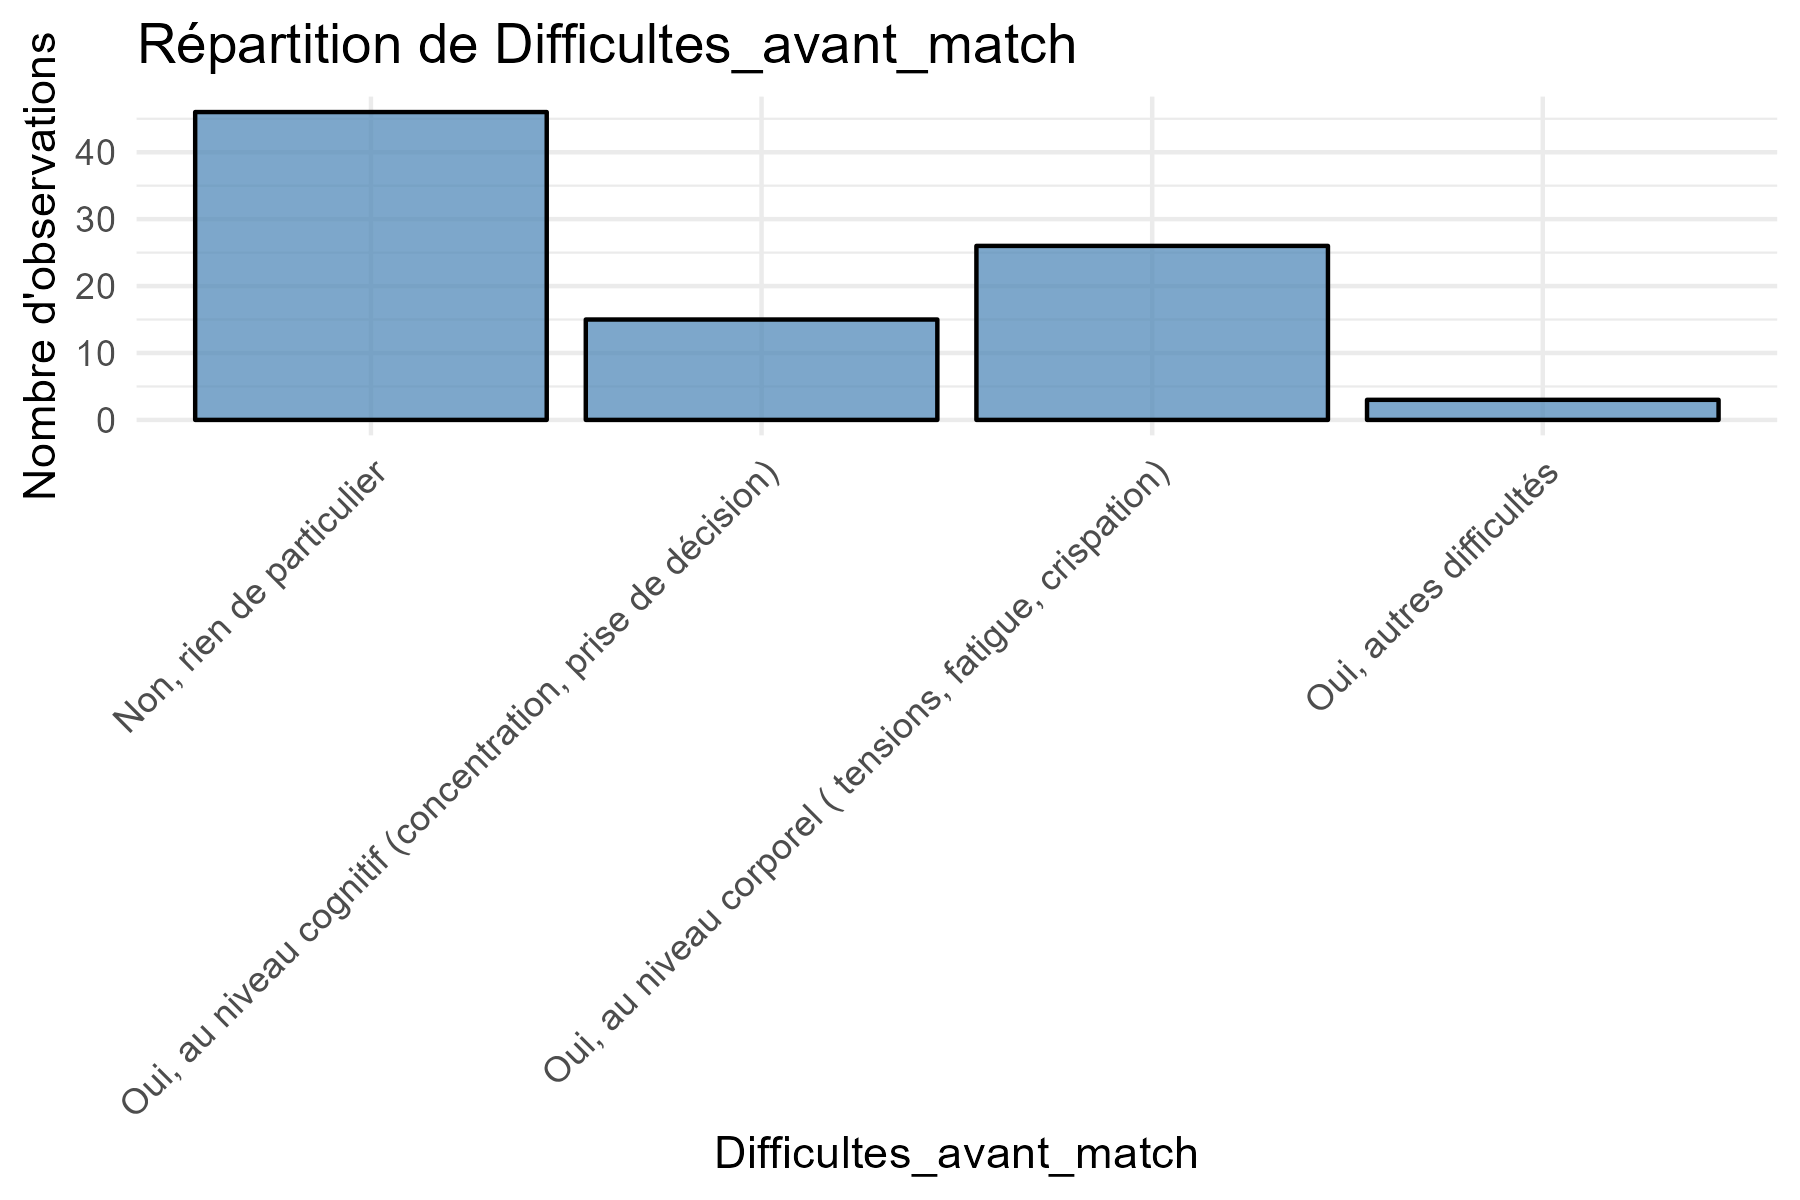
\includegraphics{Image/barplot_Difficultes_avant_match.png}
\caption{barplot difficultes avant match}
\end{figure}

\begin{figure}
\centering
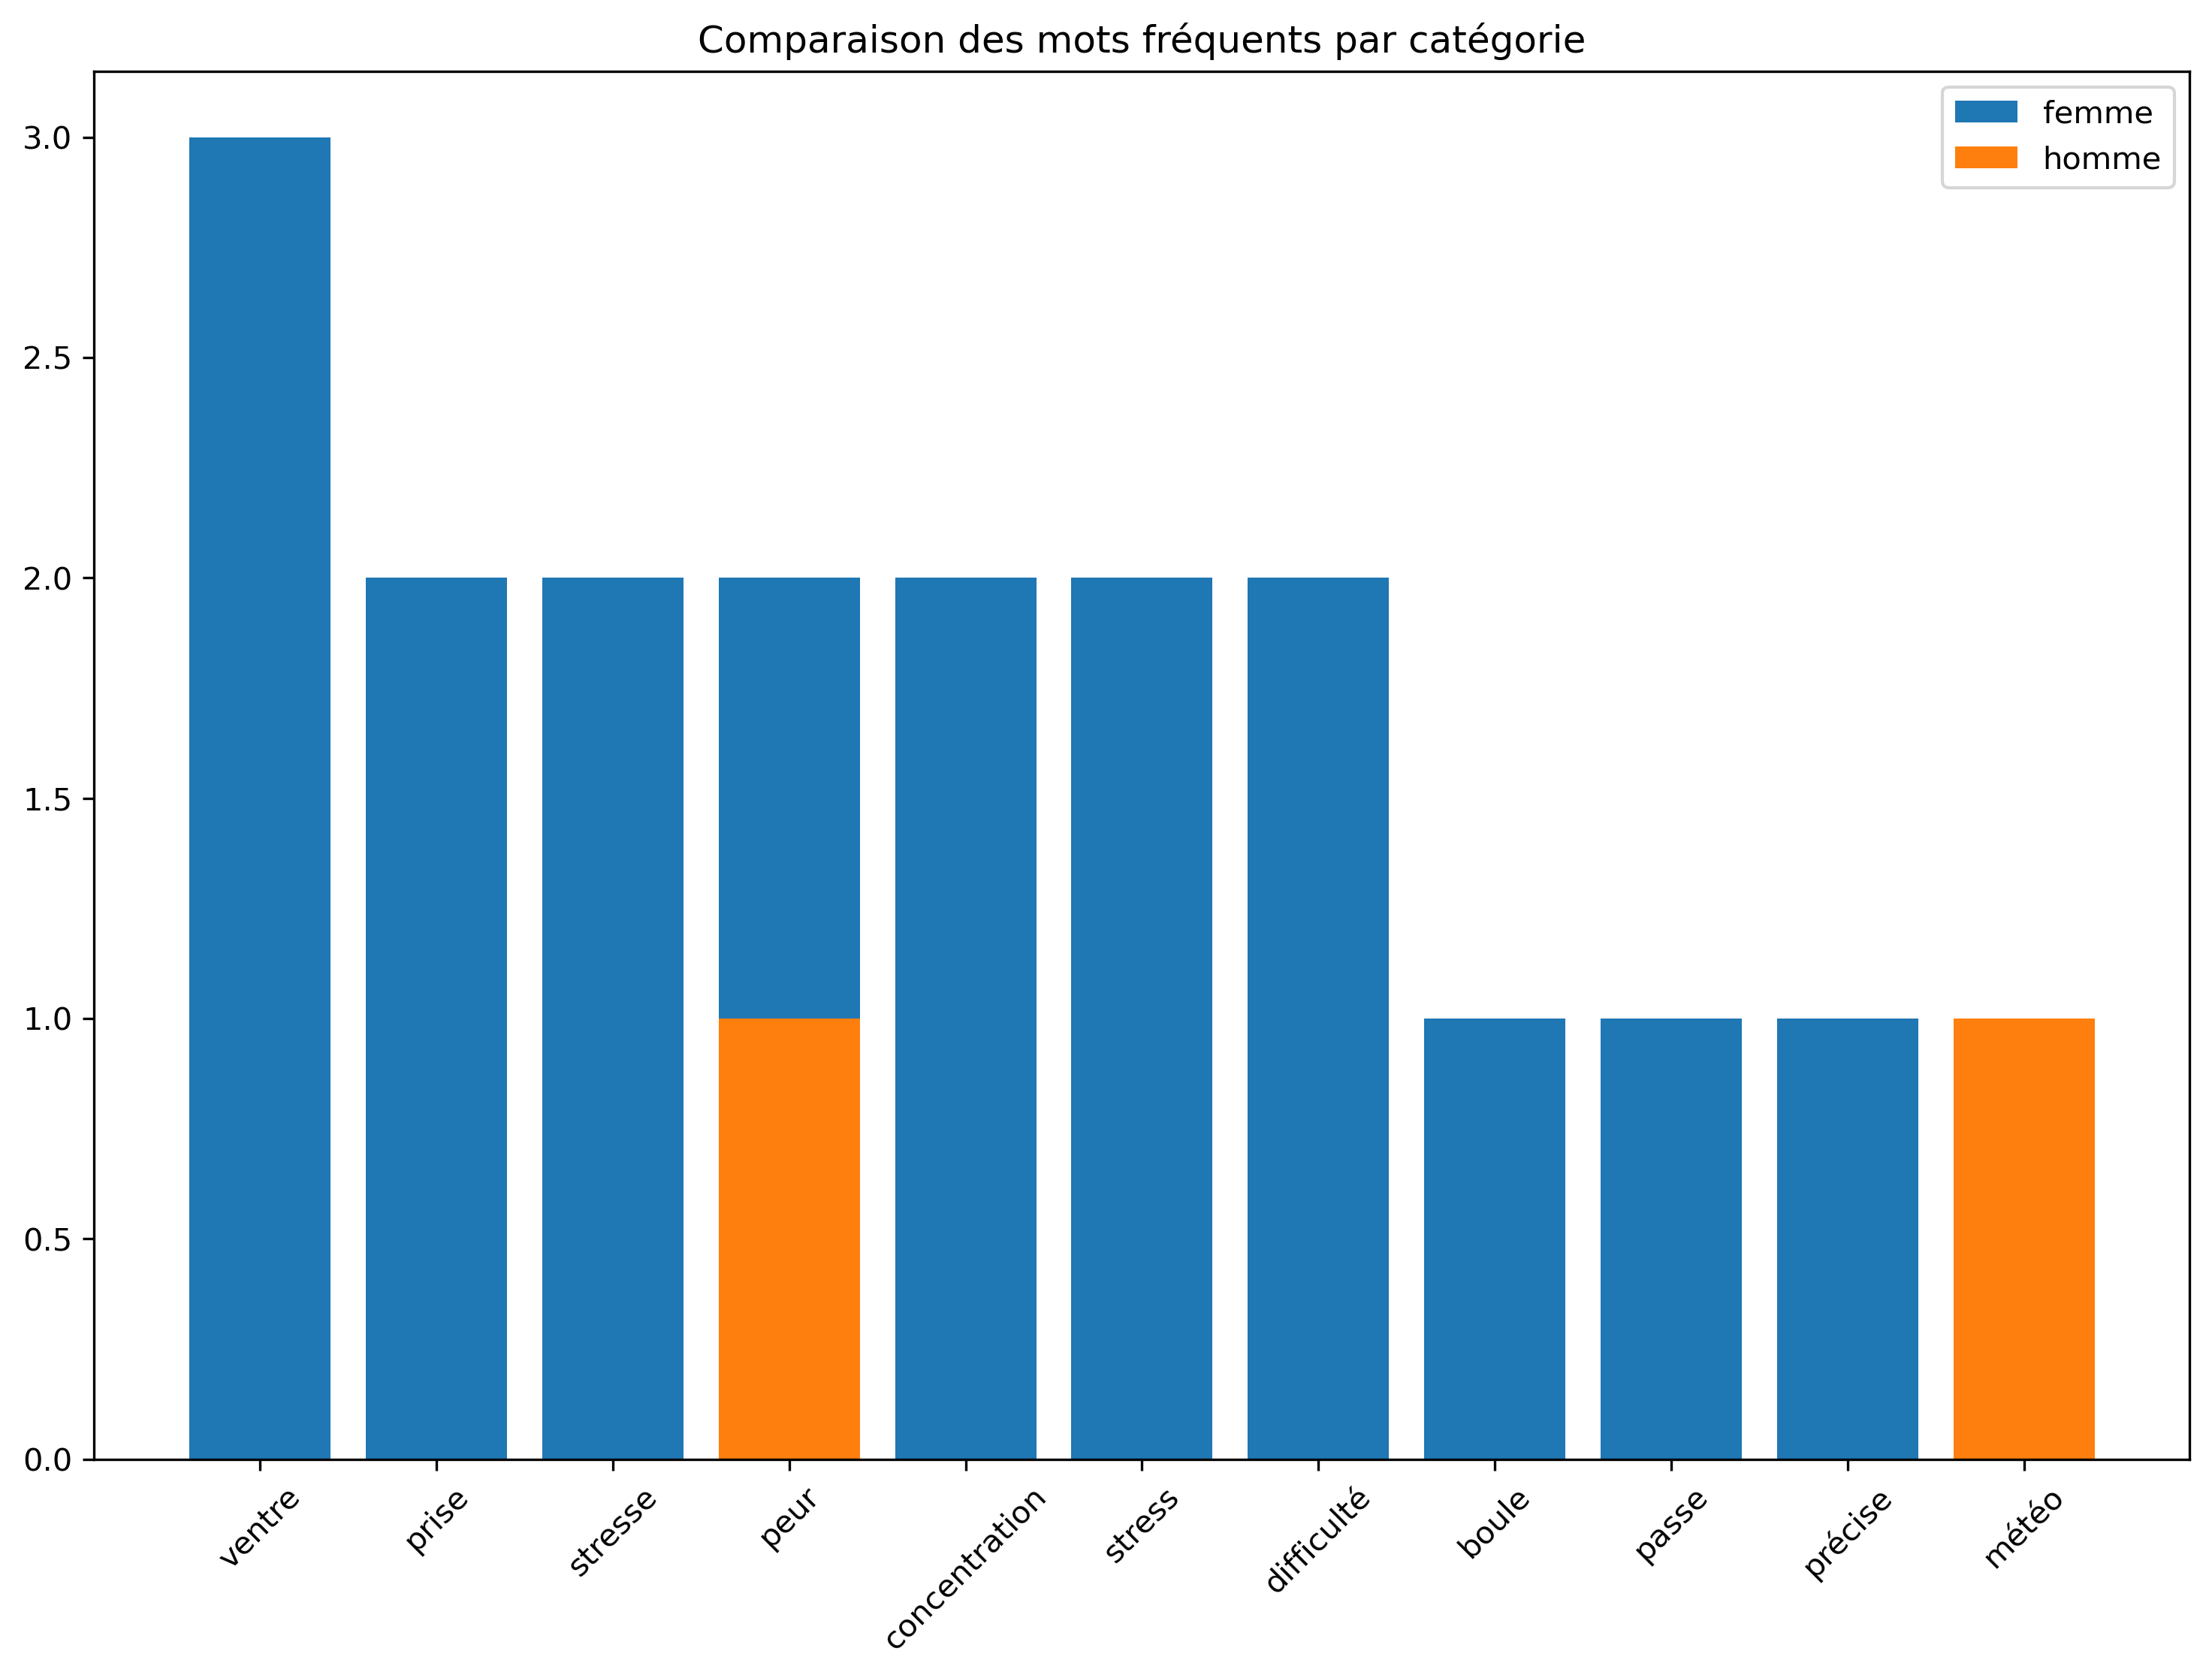
\includegraphics{Image/barplot_mots_sexe.png}
\caption{barplot}
\end{figure}

\begin{figure}
\centering
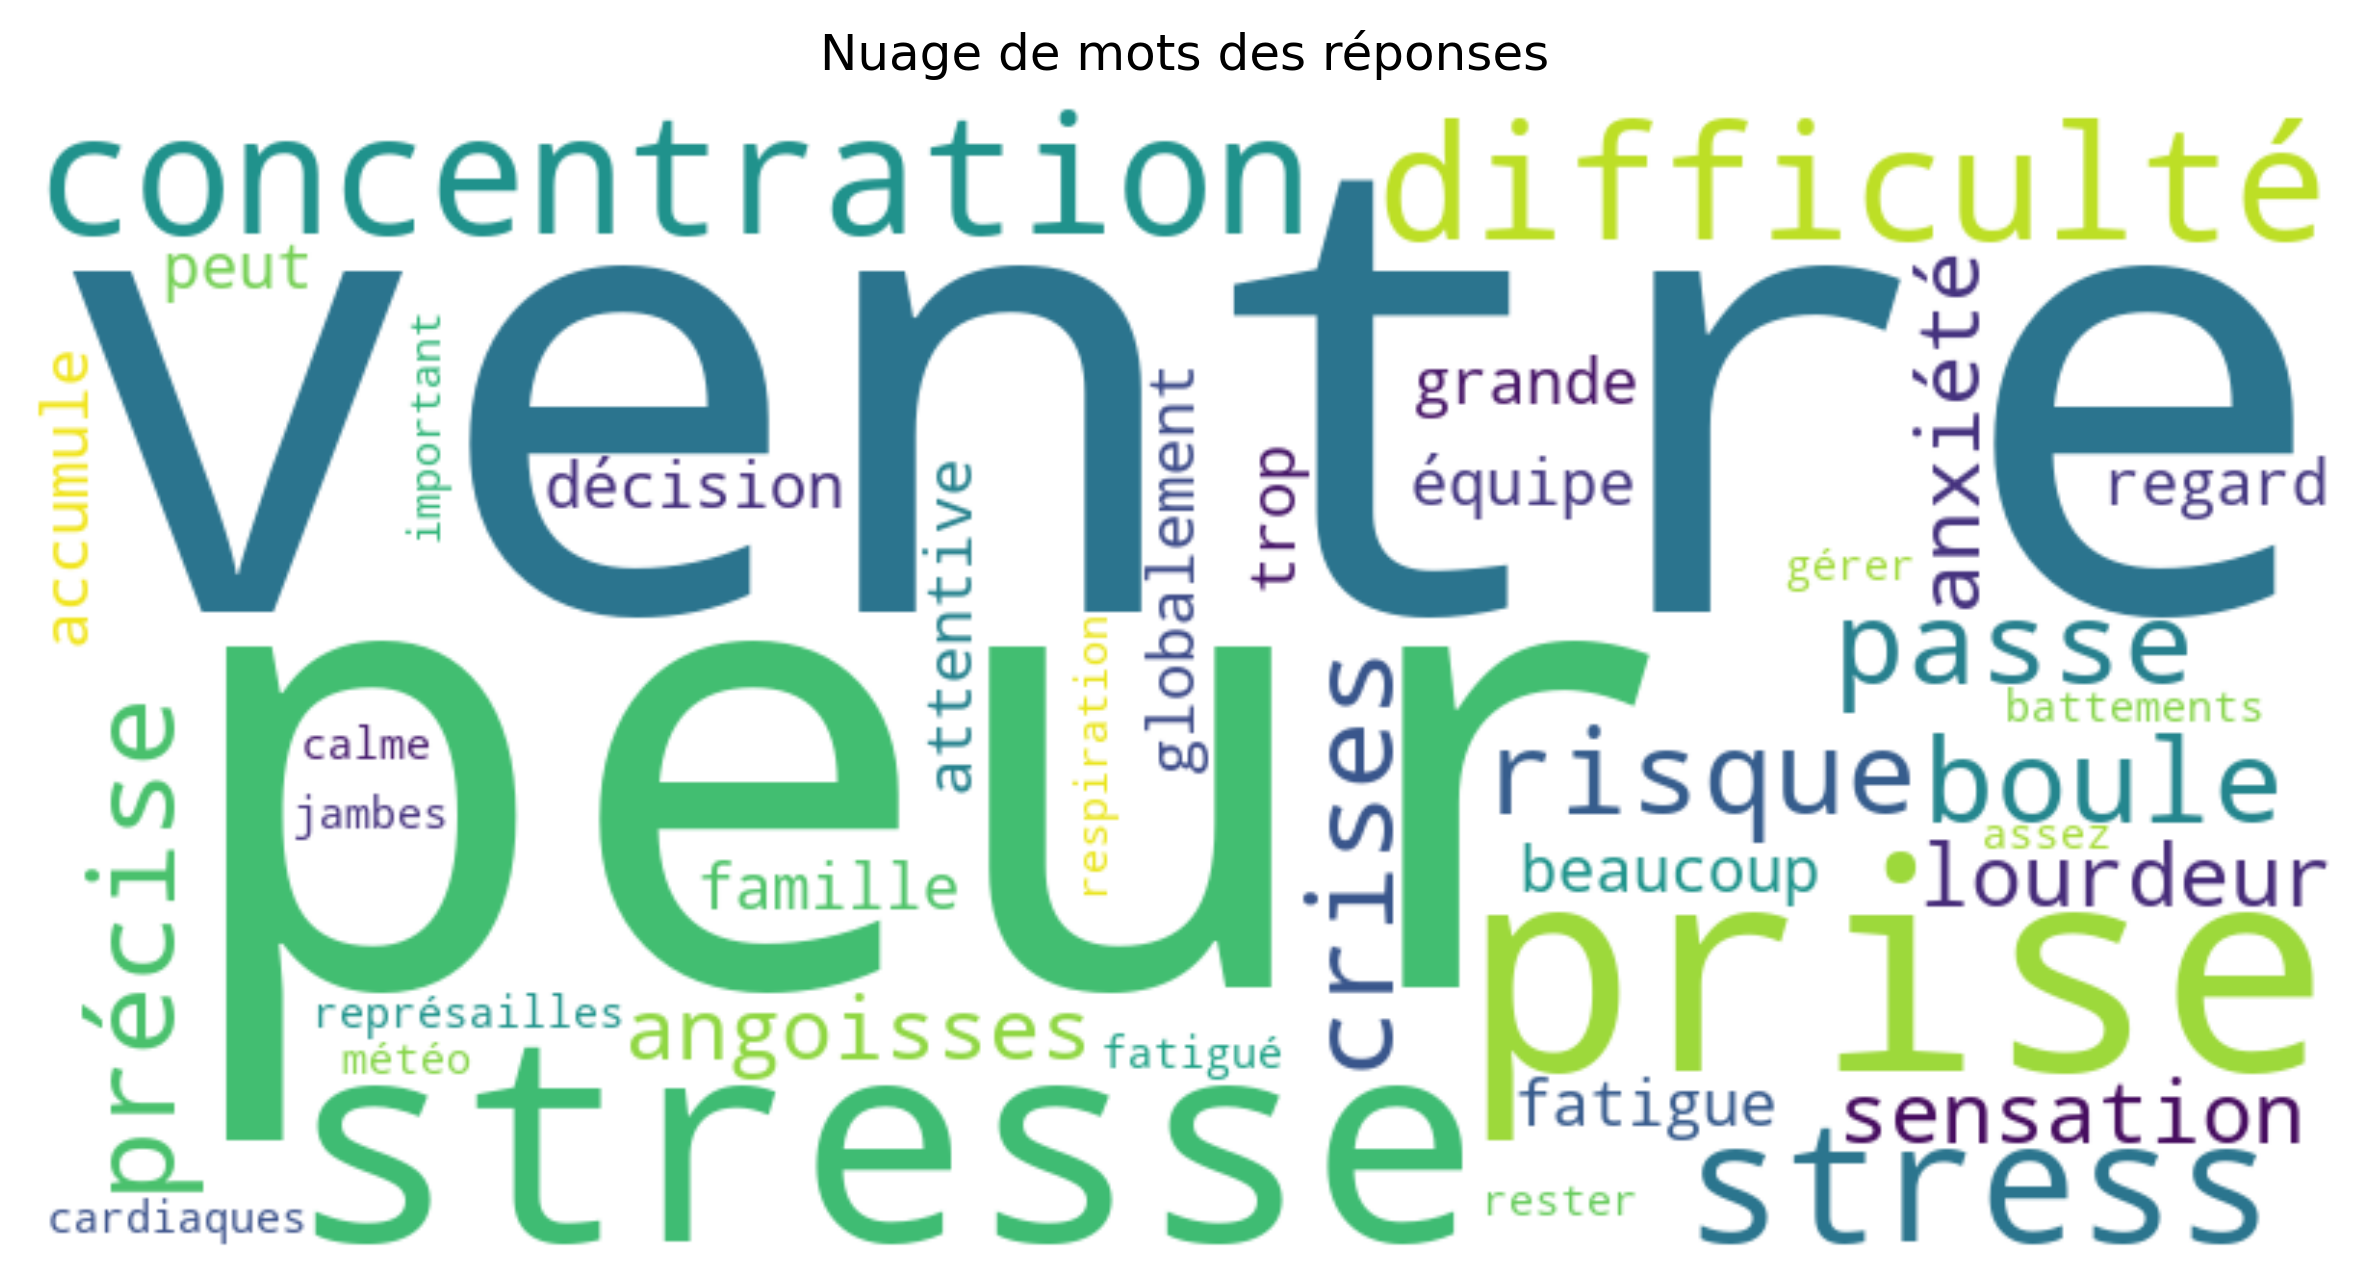
\includegraphics{Image/all_wordcloud.png}
\caption{wordcloud}
\end{figure}

\begin{figure}
\centering
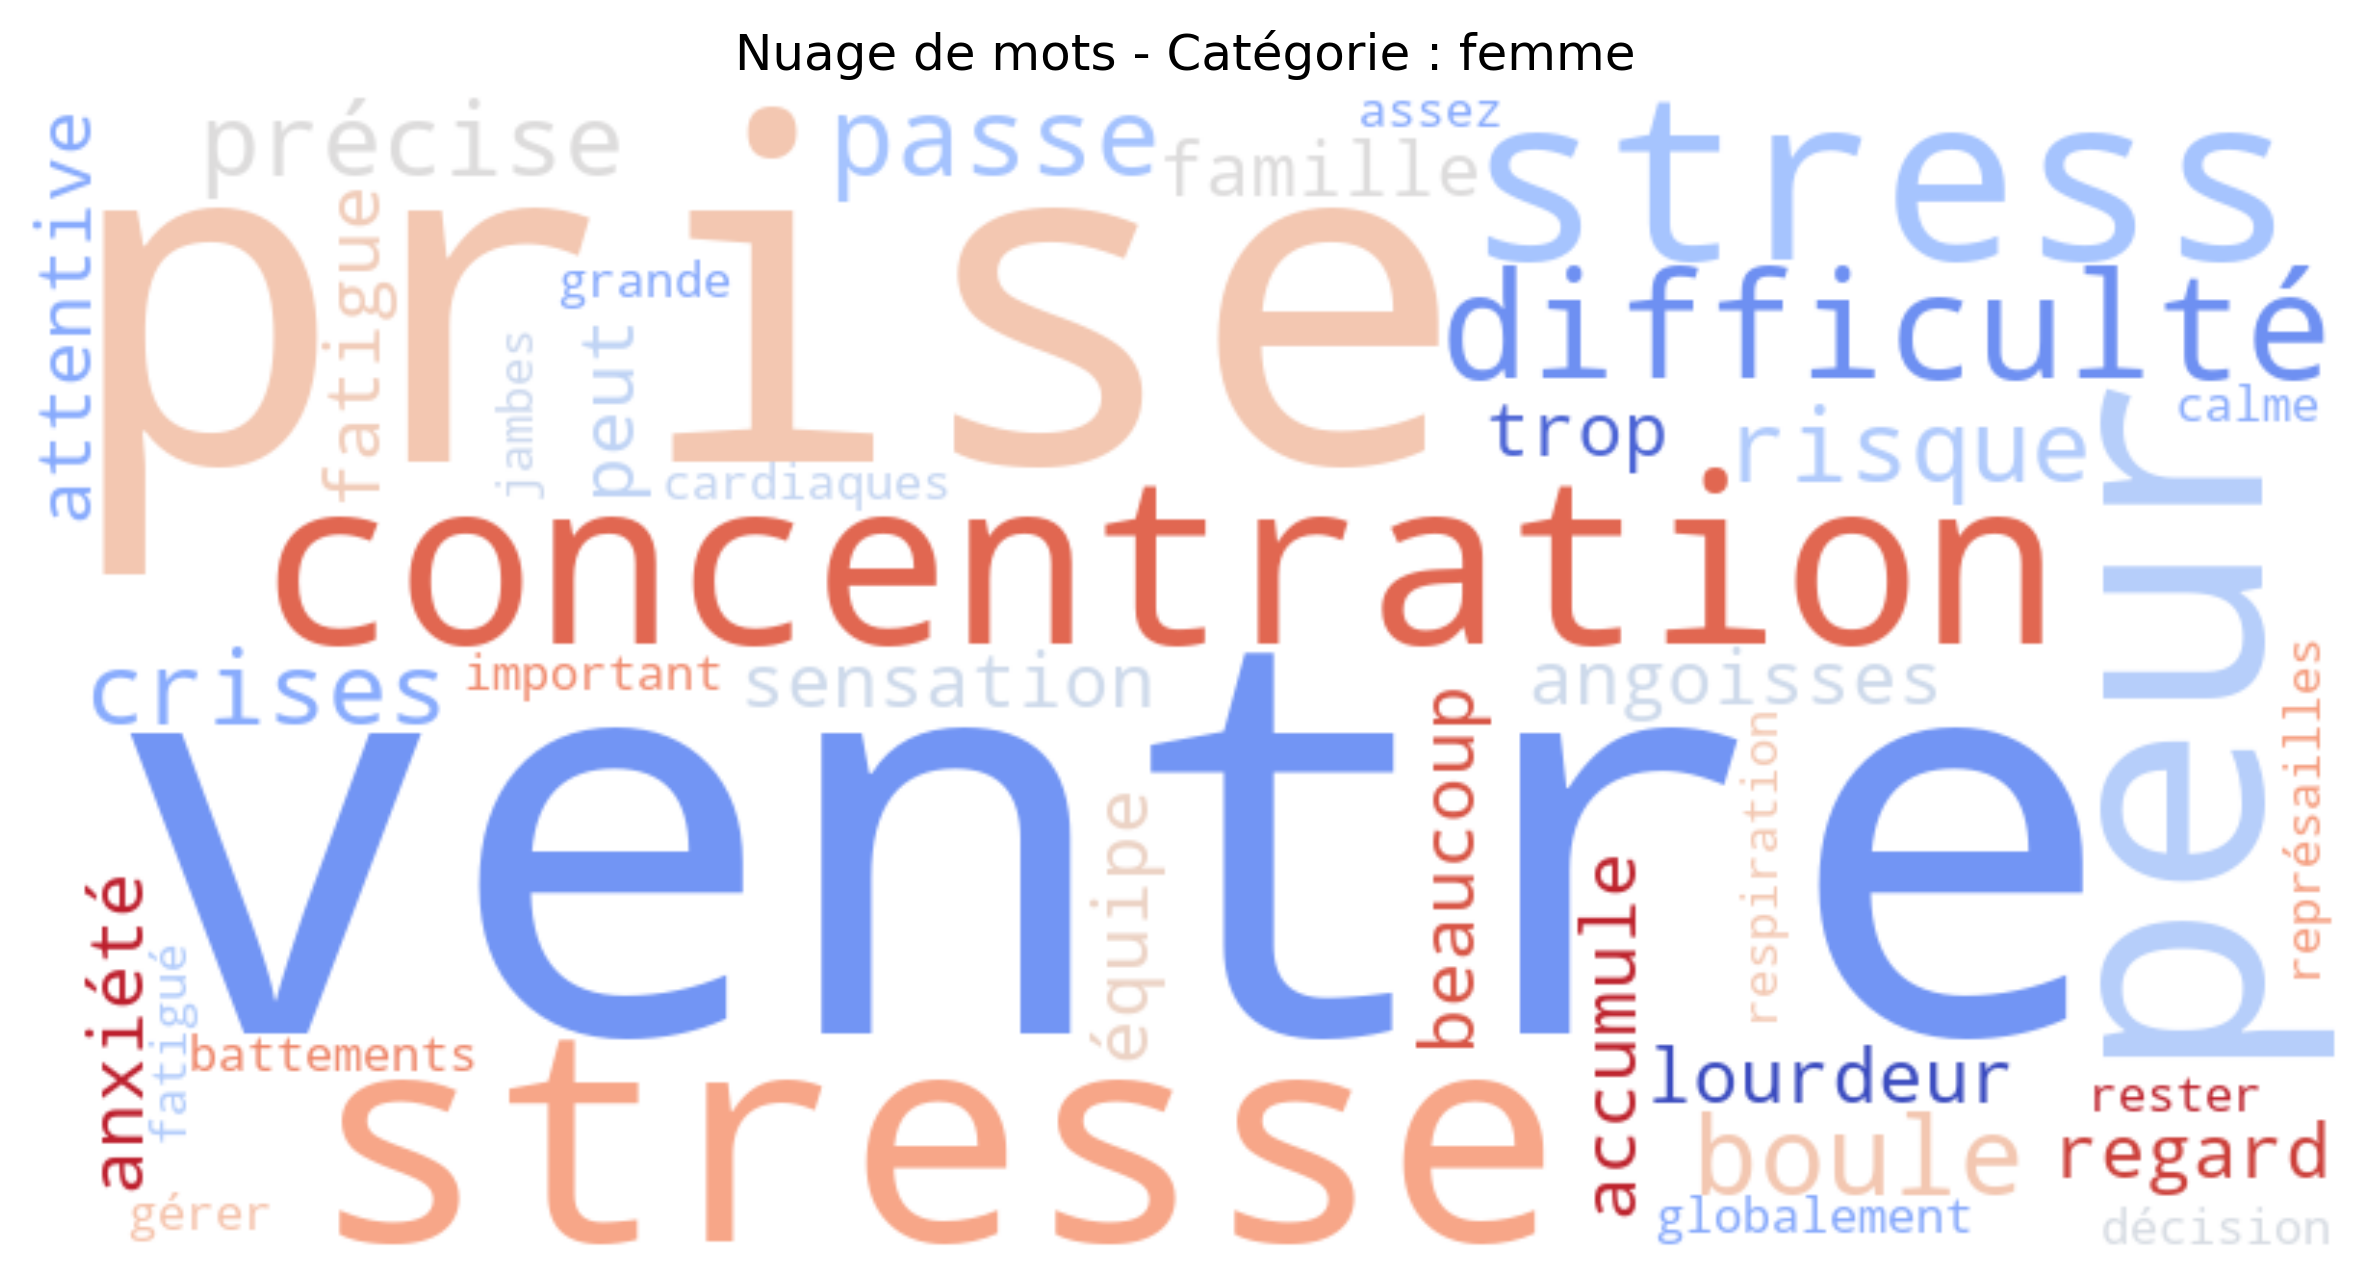
\includegraphics{Image/wordcloud_femme.png}
\caption{wordcloud femme}
\end{figure}

\begin{figure}
\centering
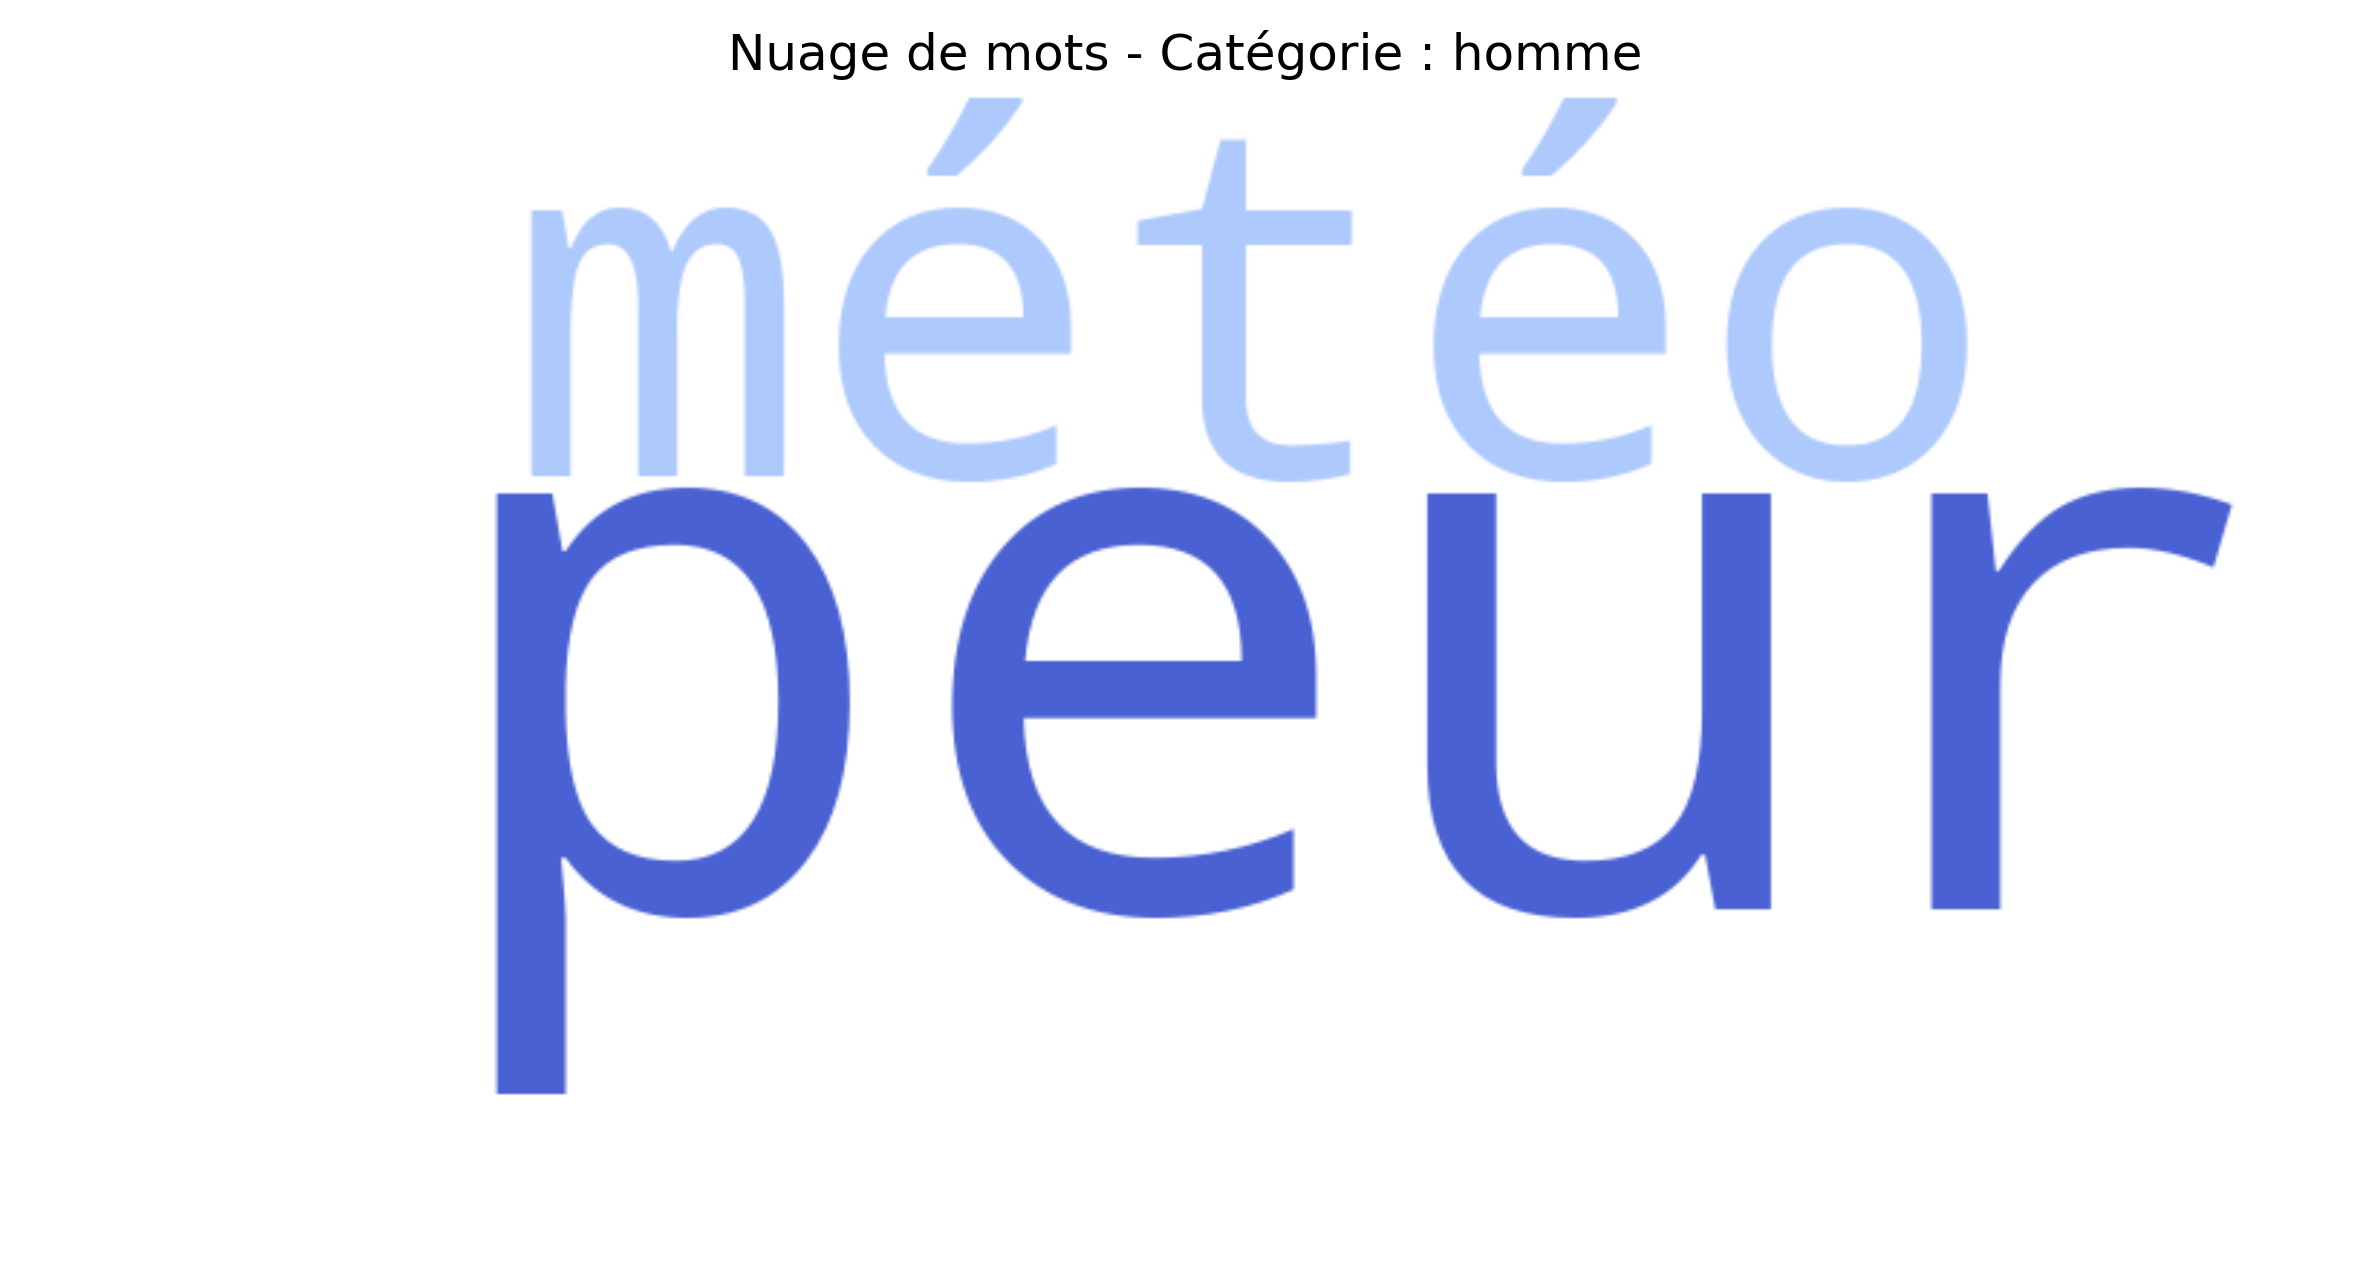
\includegraphics{Image/wordcloud_homme.png}
\caption{wordcloud homme}
\end{figure}

\section{affirmation 1}\label{affirmation-1}

affirmation 1

\begin{figure}
\centering
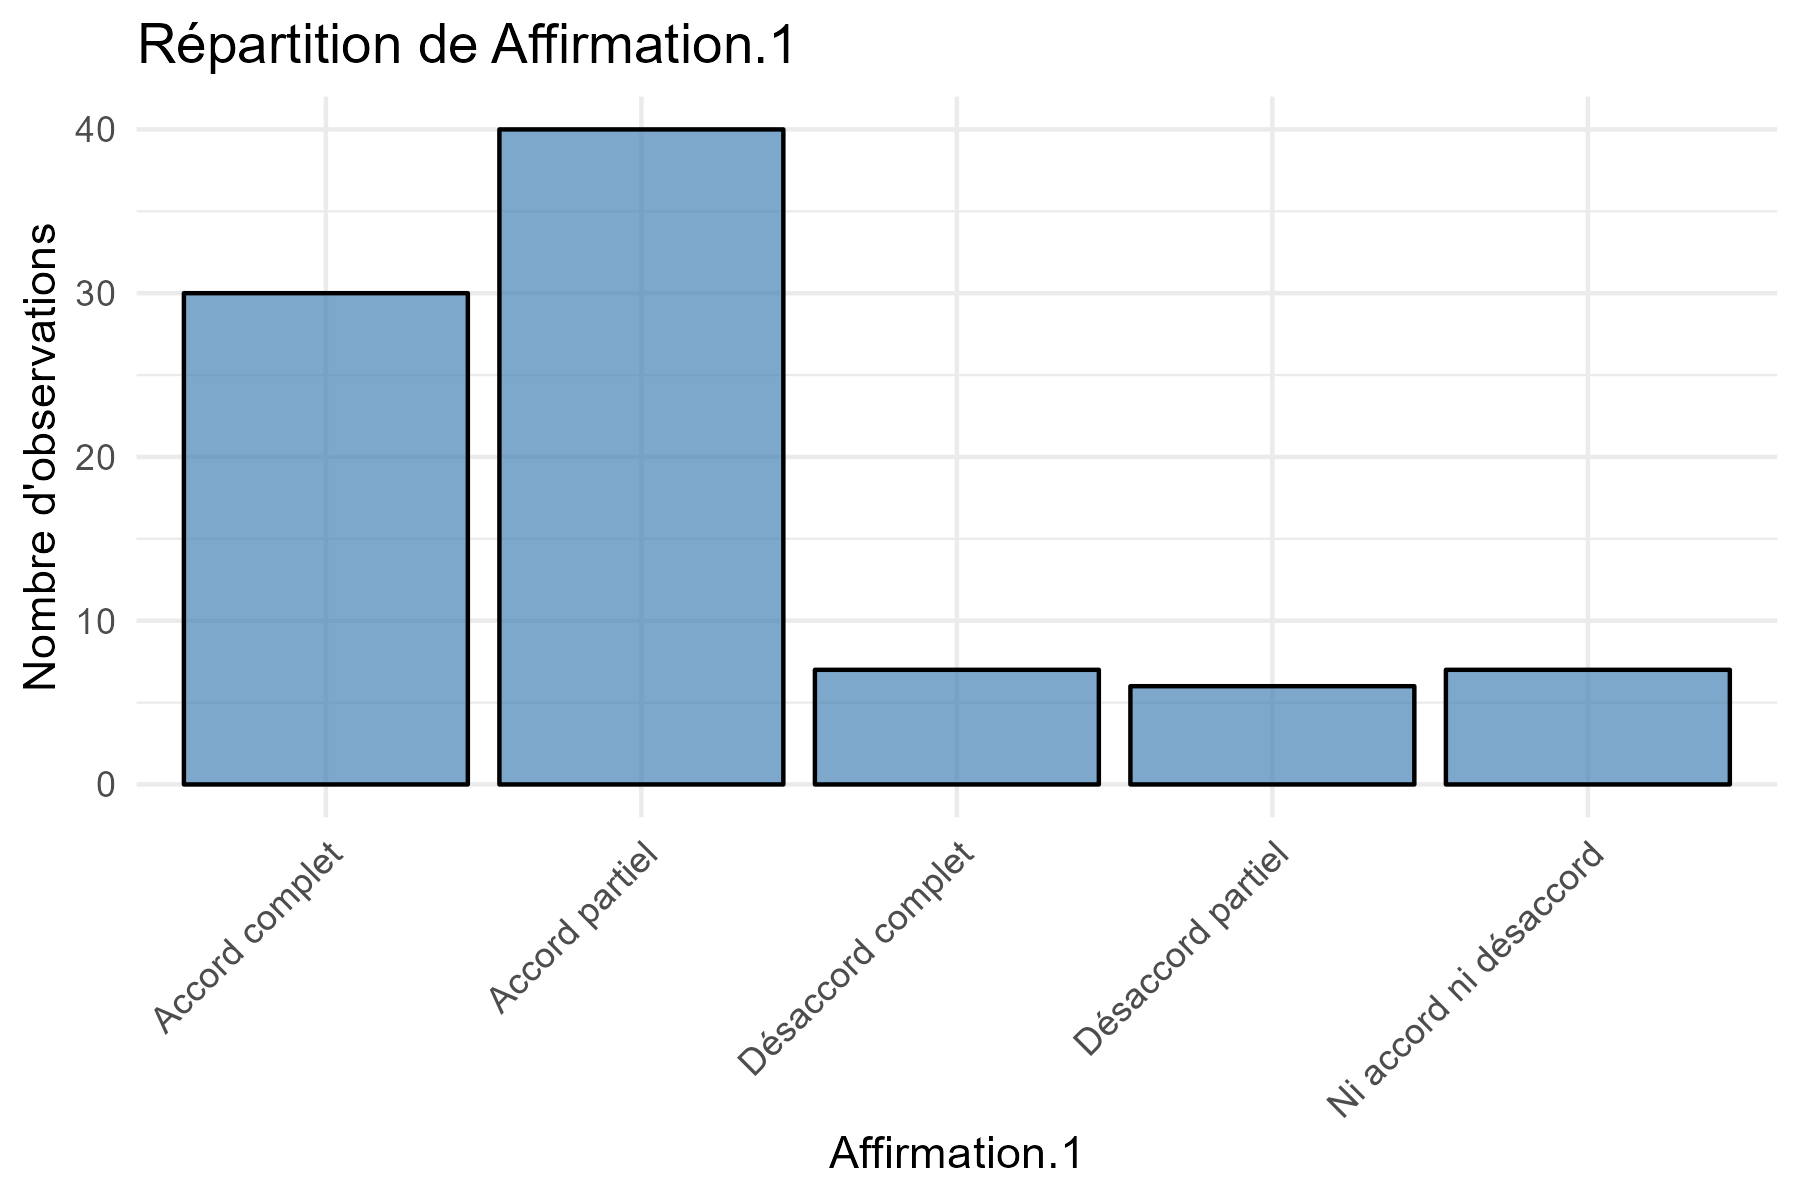
\includegraphics{Image/barplot_Affirmation.1.png}
\caption{barplot affirmation 1}
\end{figure}

\section{affirmation 12}\label{affirmation-12}

affirmation 12

\begin{figure}
\centering
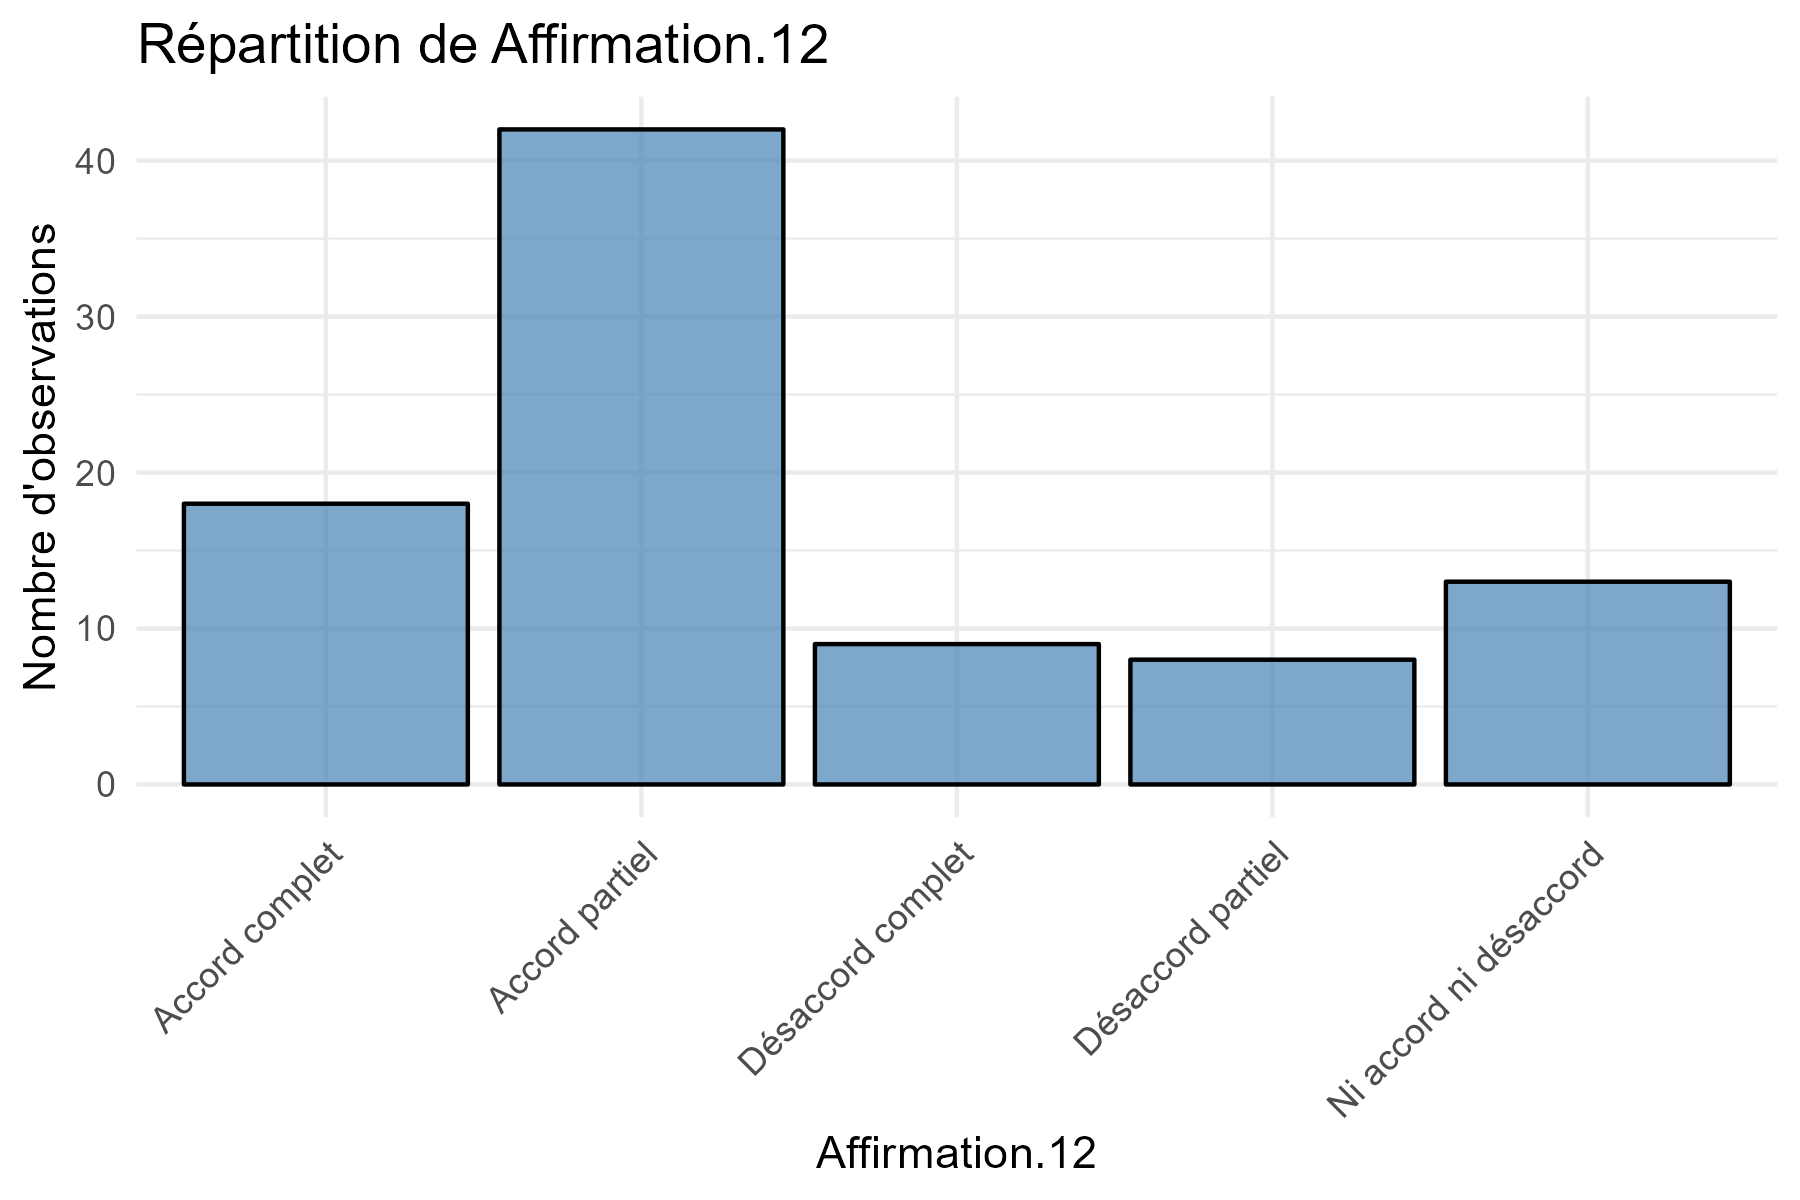
\includegraphics{Image/barplot_Affirmation.12.png}
\caption{barplot affirmation 12}
\end{figure}

\section{affirmation 13}\label{affirmation-13}

affirmation 13

\begin{figure}
\centering
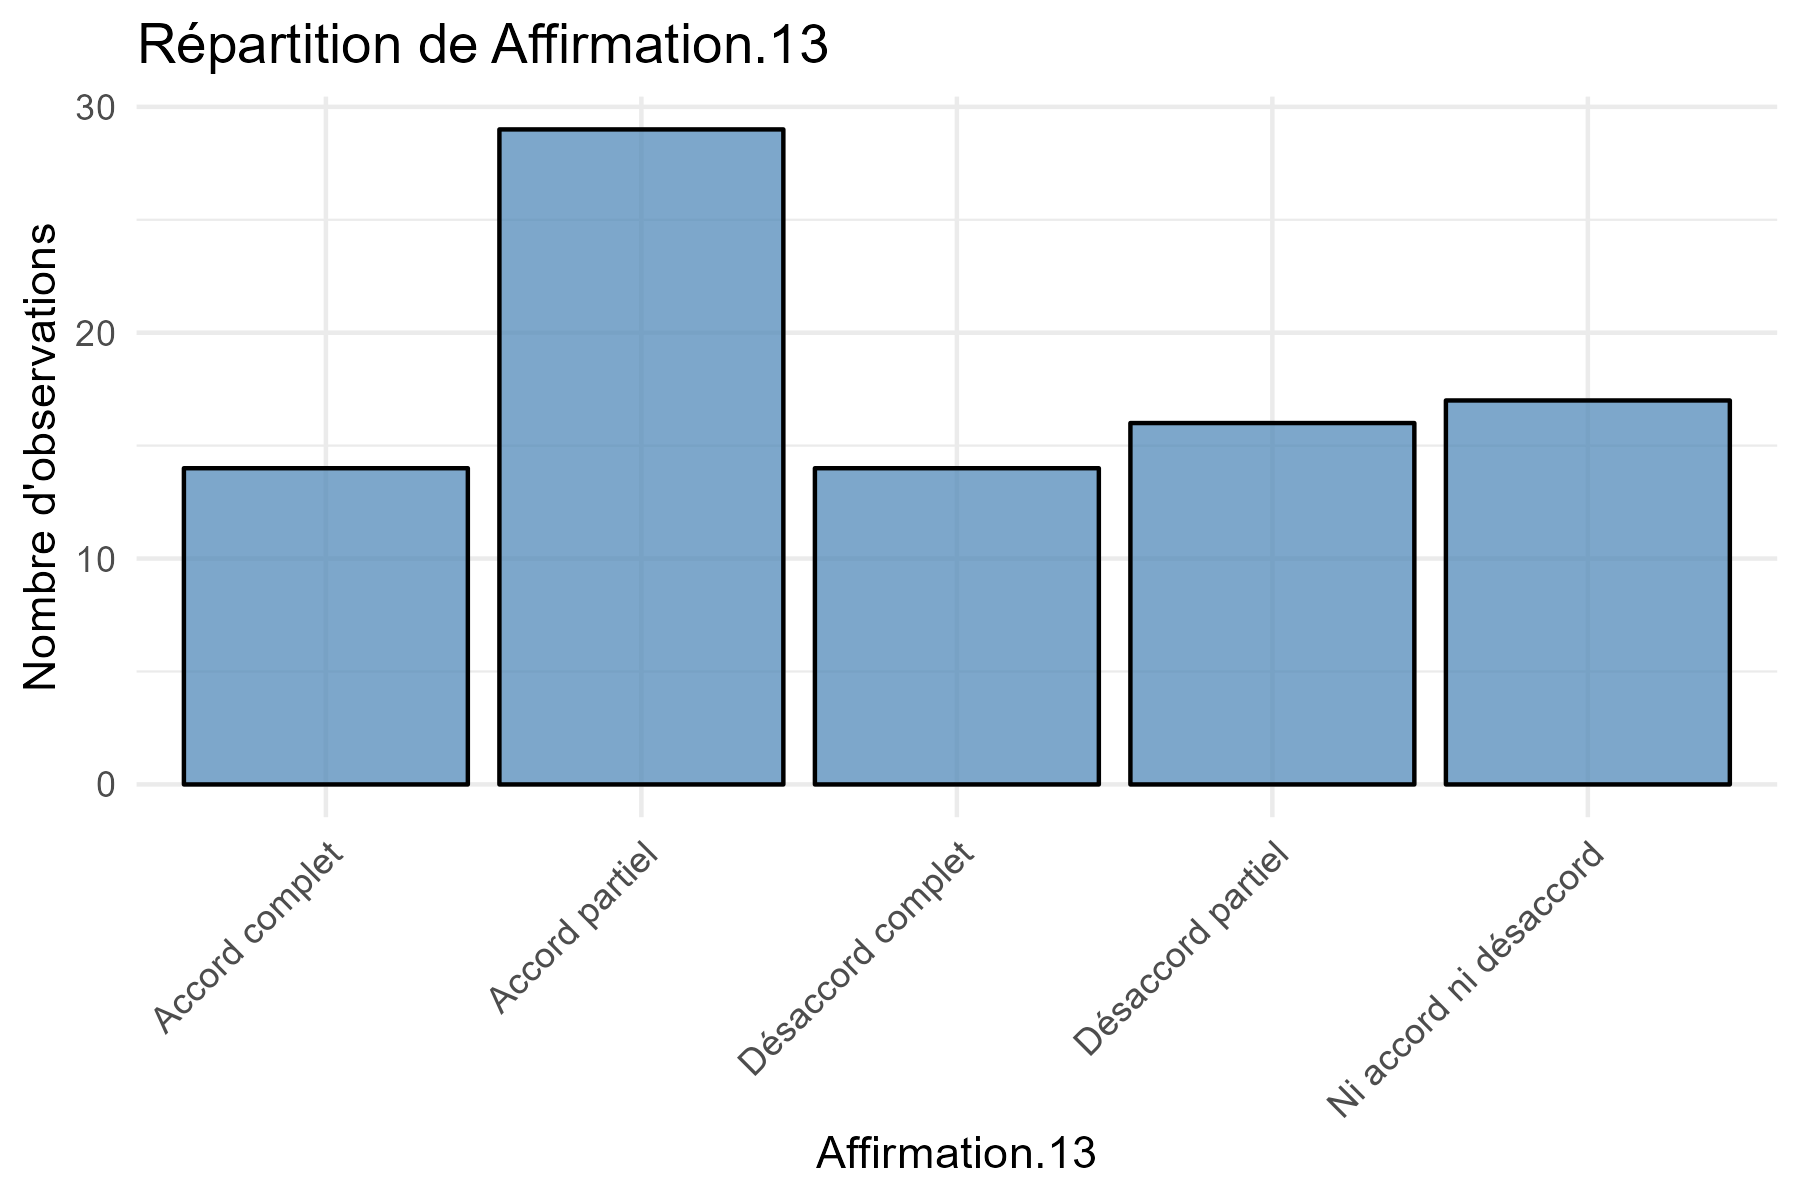
\includegraphics{Image/barplot_Affirmation.13.png}
\caption{barplot affirmation 13}
\end{figure}

\section{affirmation 14}\label{affirmation-14}

affirmation 14

\begin{figure}
\centering
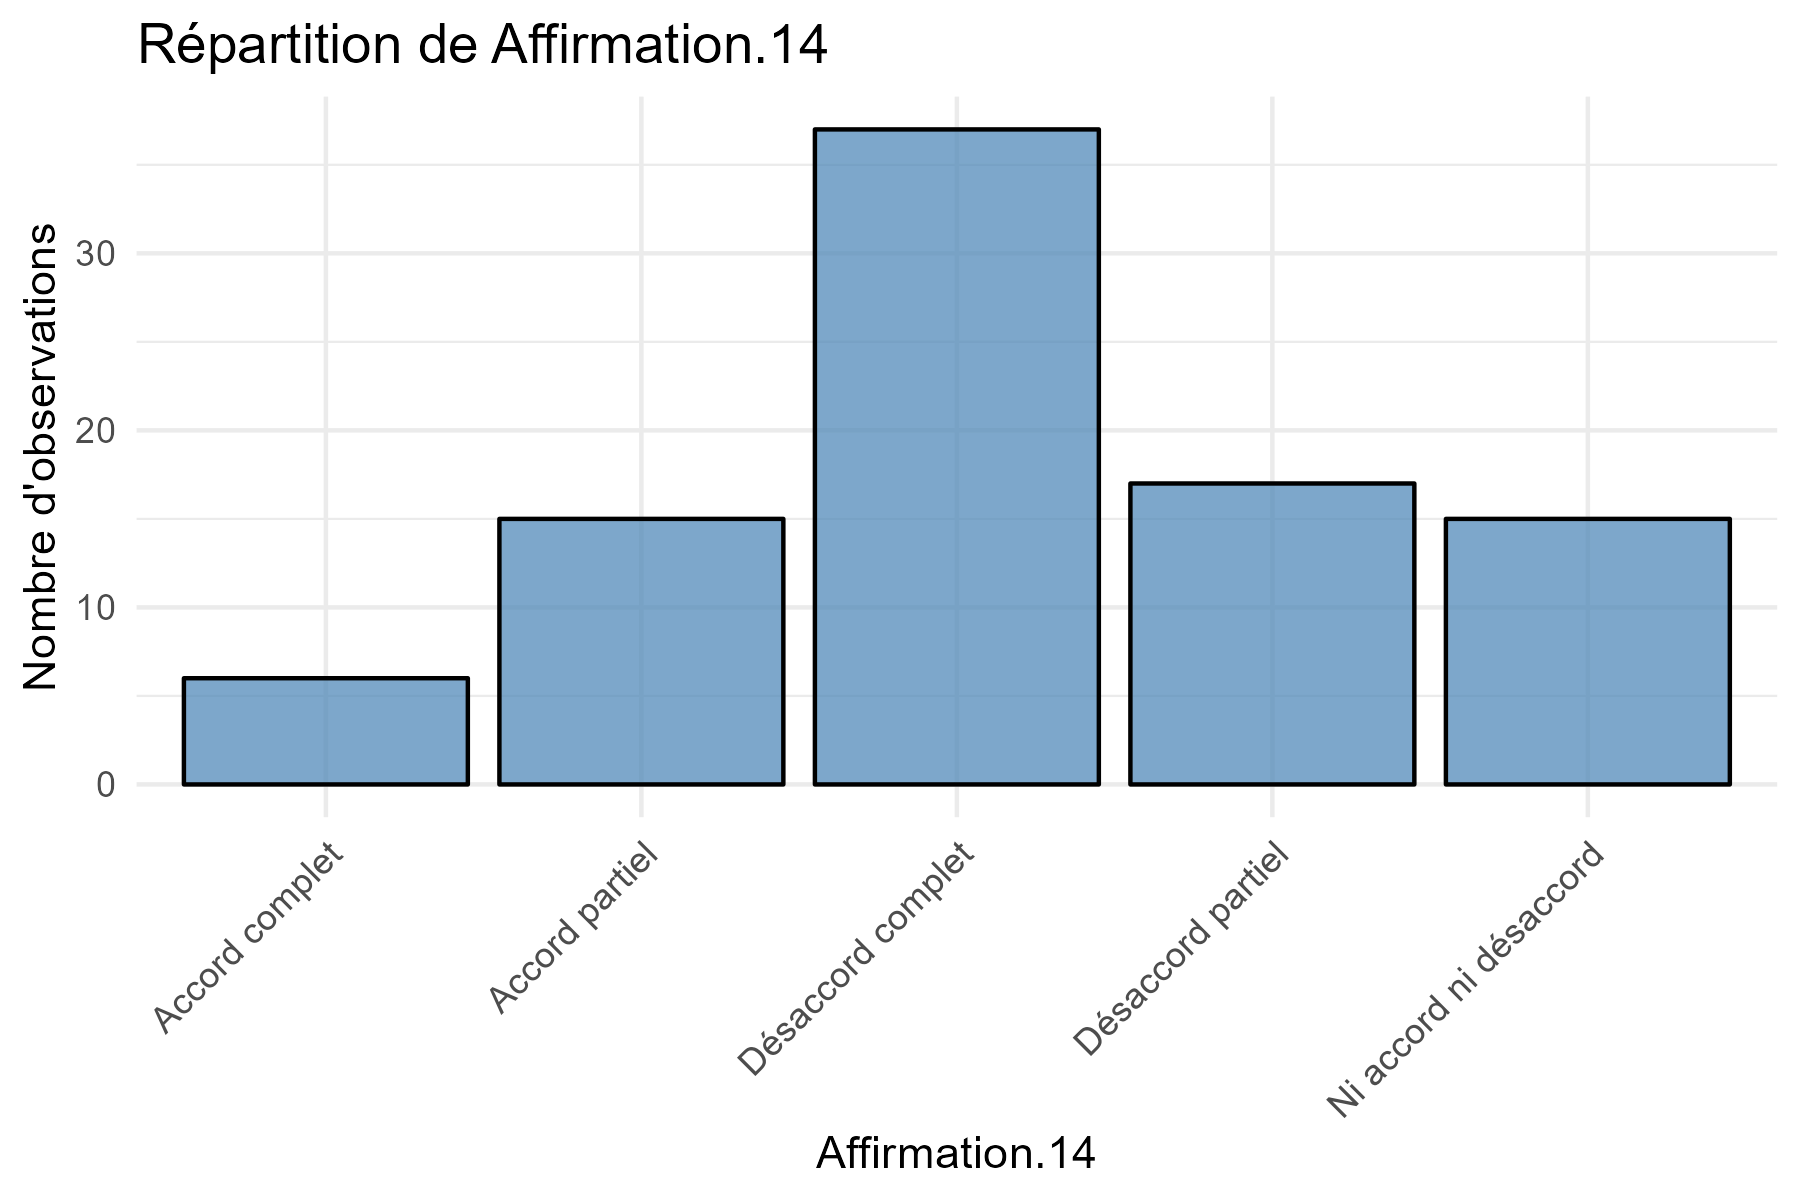
\includegraphics{Image/barplot_Affirmation.14.png}
\caption{barplot affirmation 14}
\end{figure}

\section{affirmation 15}\label{affirmation-15}

affirmation 15

\begin{figure}
\centering
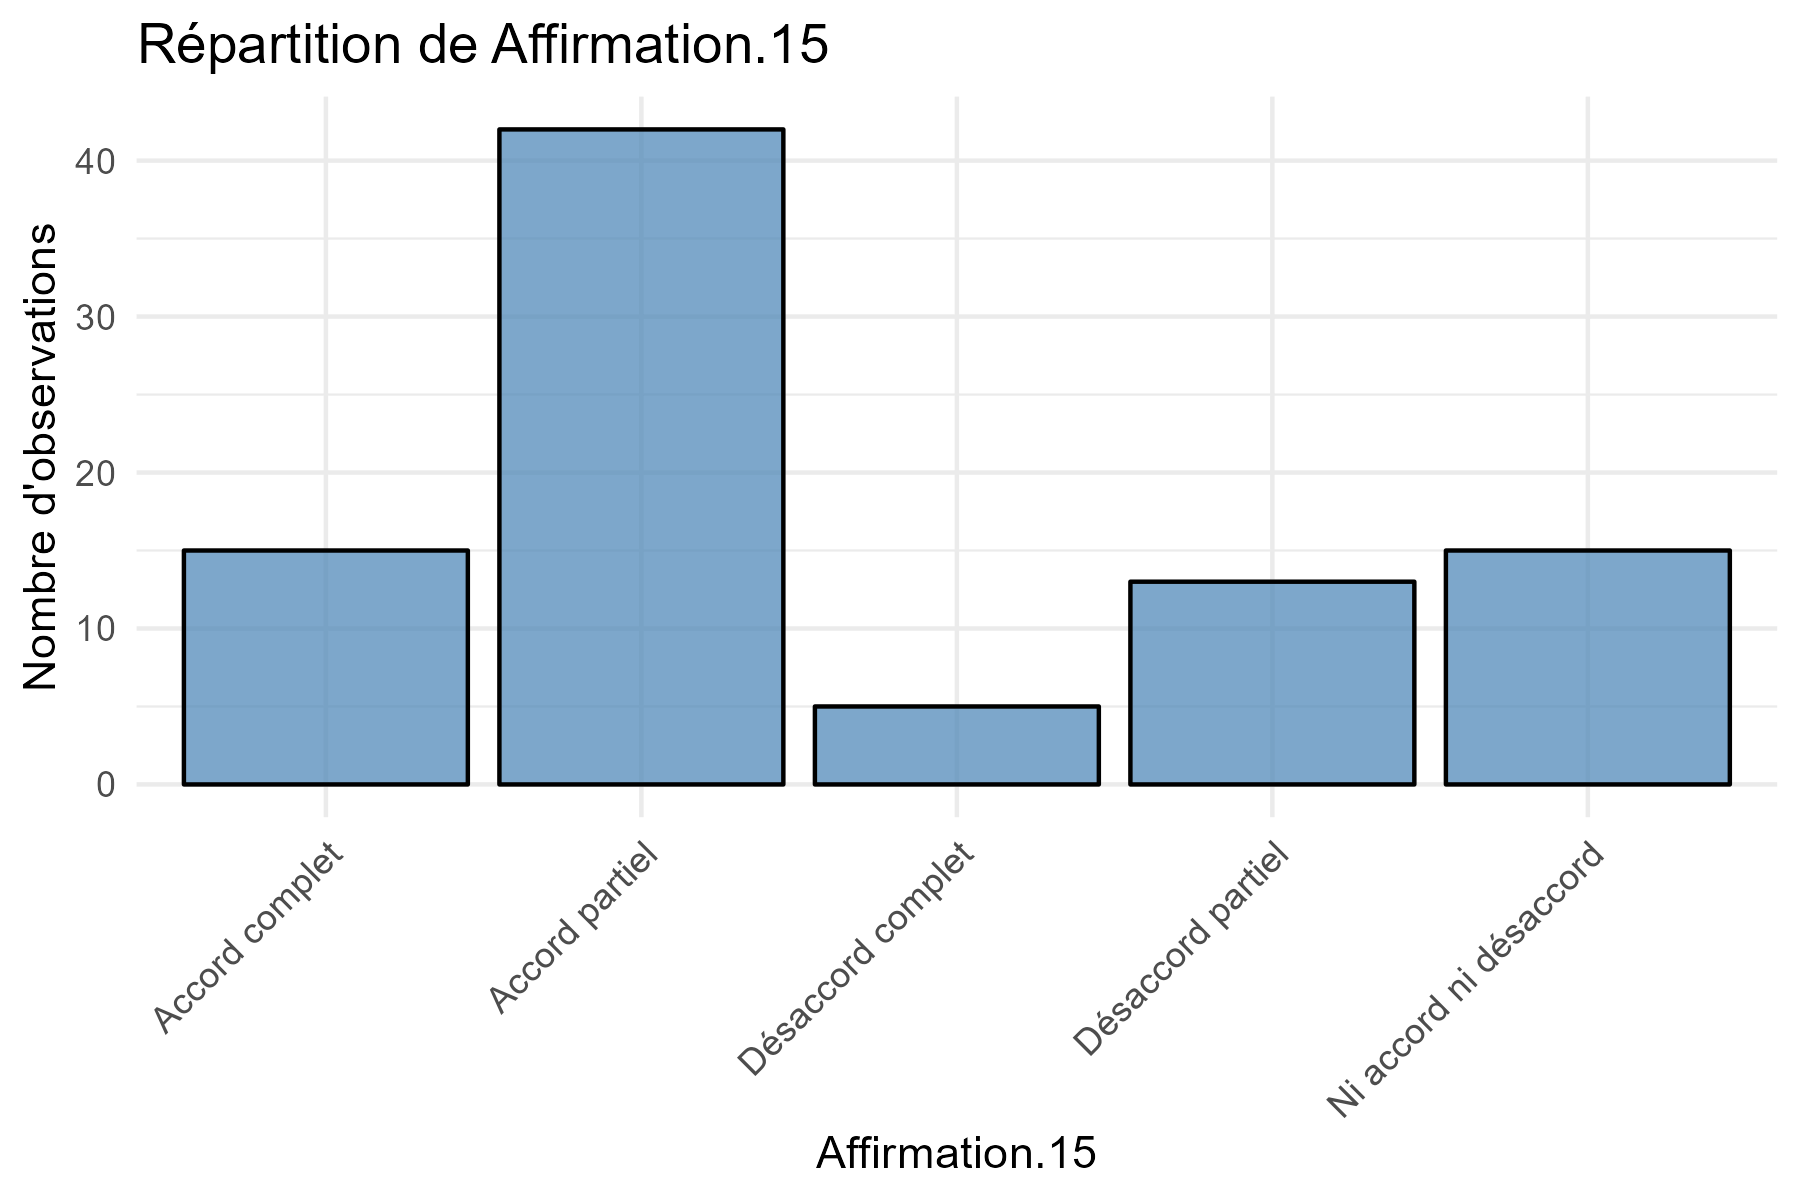
\includegraphics{Image/barplot_Affirmation.15.png}
\caption{barplot affirmation 15}
\end{figure}

\section{affirmation 16}\label{affirmation-16}

affirmation 16

\begin{figure}
\centering
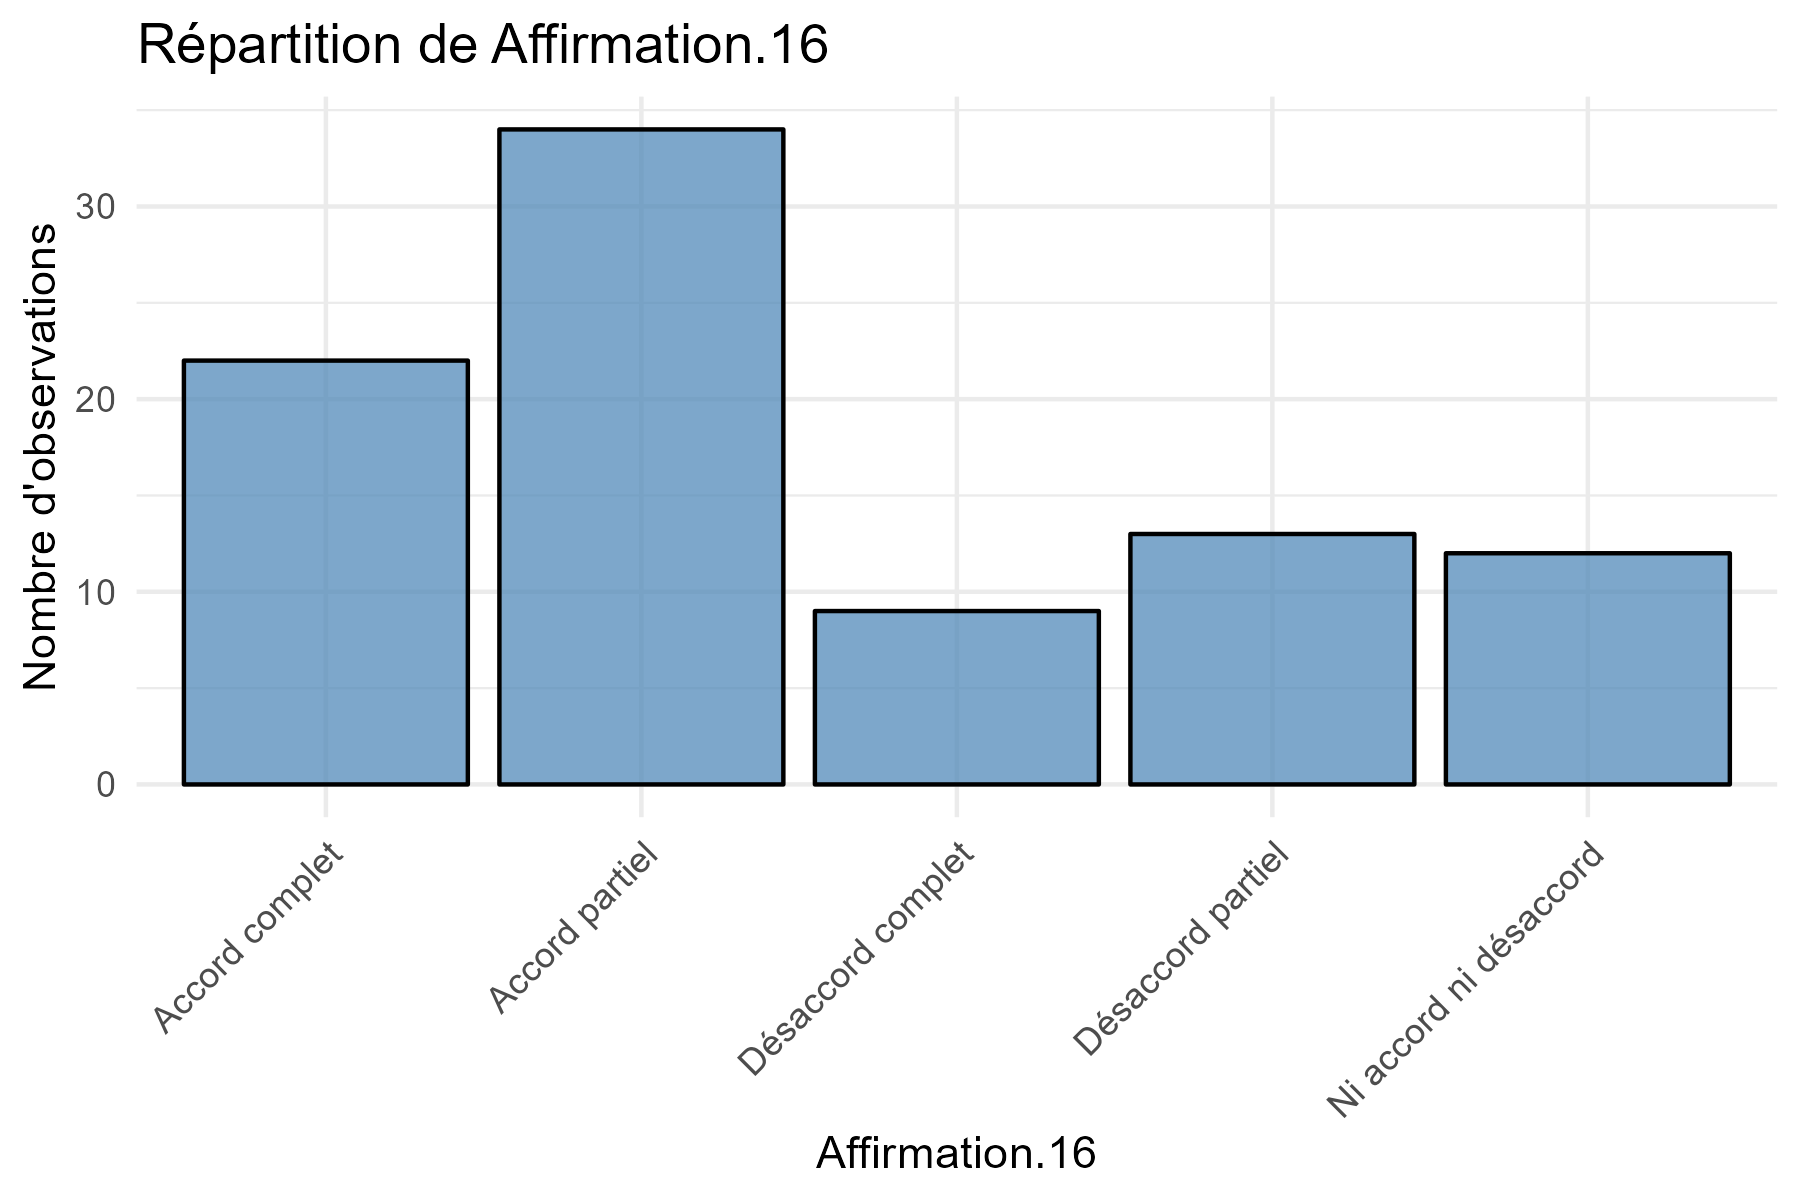
\includegraphics{Image/barplot_Affirmation.16.png}
\caption{barplot affirmation 16}
\end{figure}

\section{affirmation 17}\label{affirmation-17}

affirmation 17

\begin{figure}
\centering
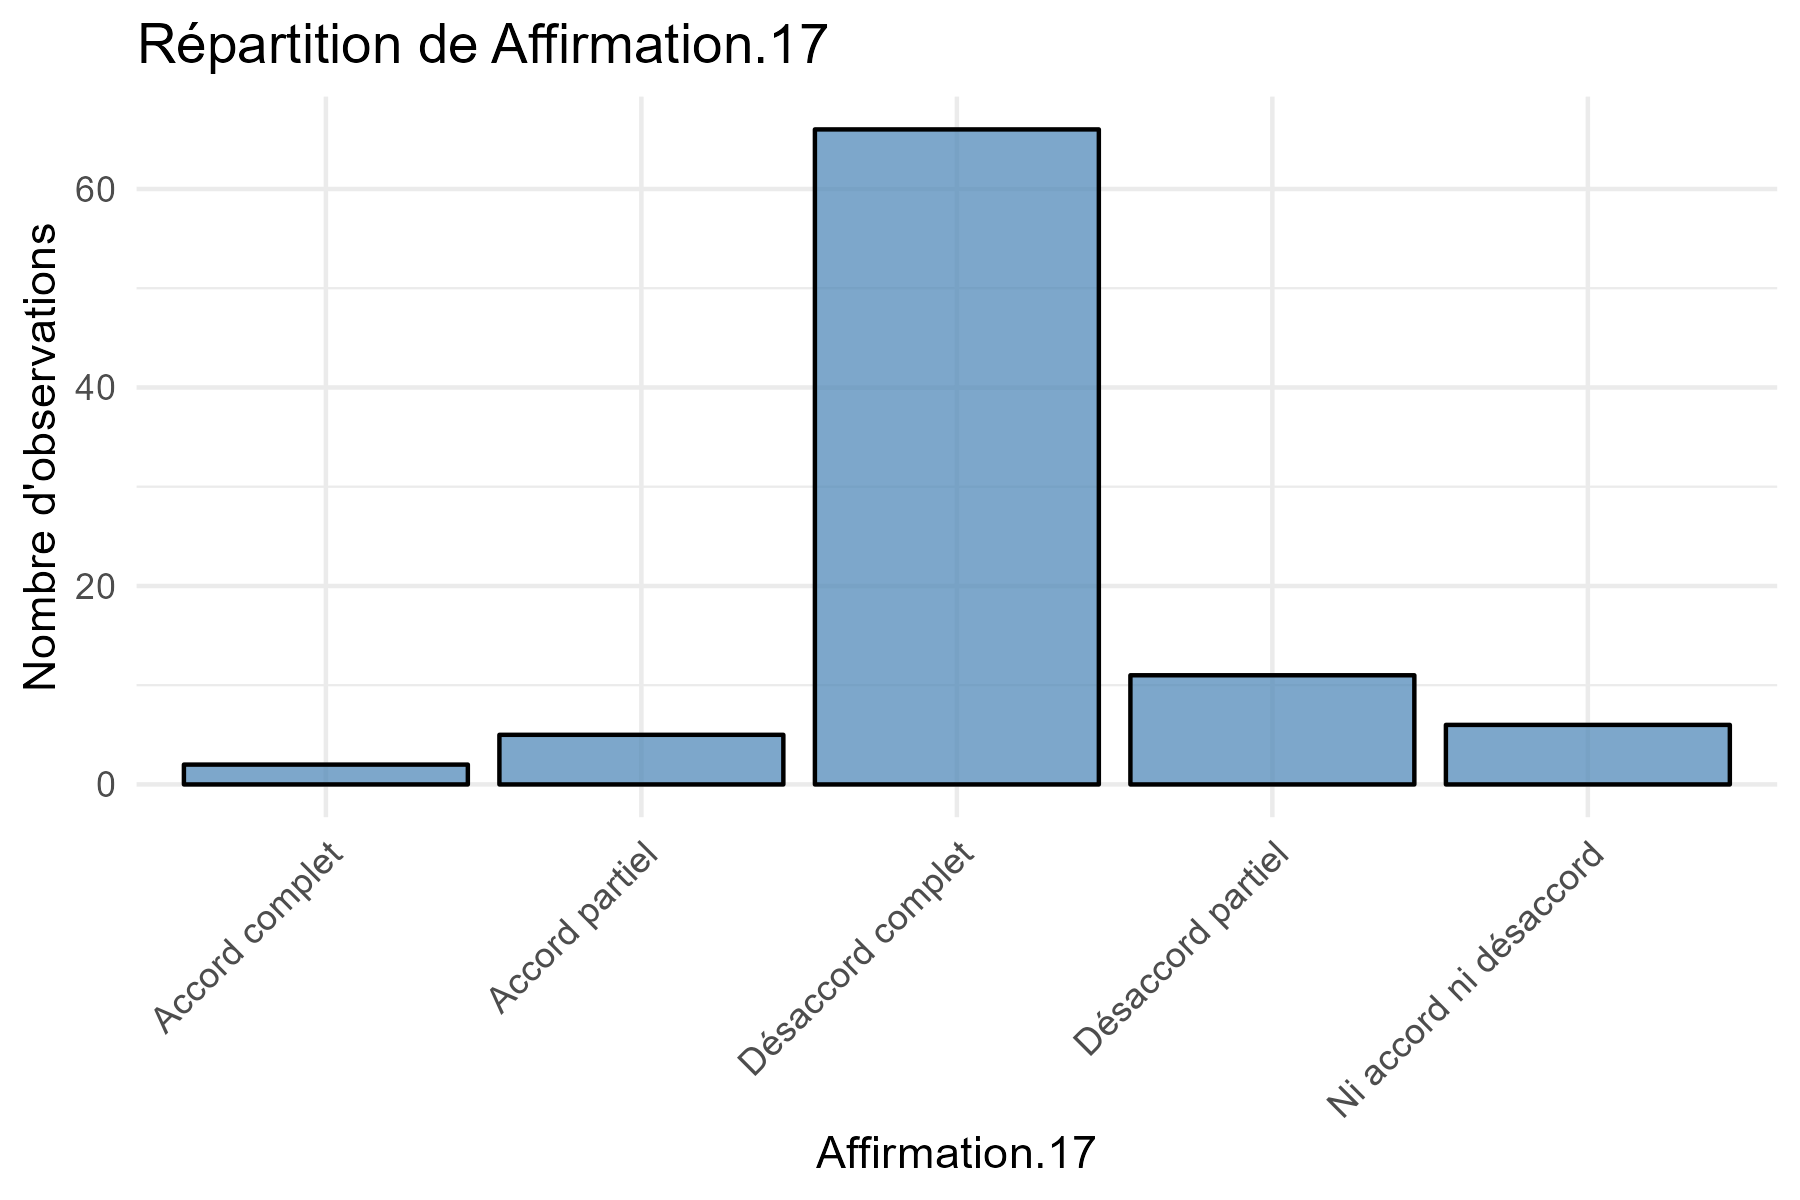
\includegraphics{Image/barplot_Affirmation.17.png}
\caption{barplot affirmation 17}
\end{figure}

\section{affirmation 18}\label{affirmation-18}

affirmation 18

\begin{figure}
\centering
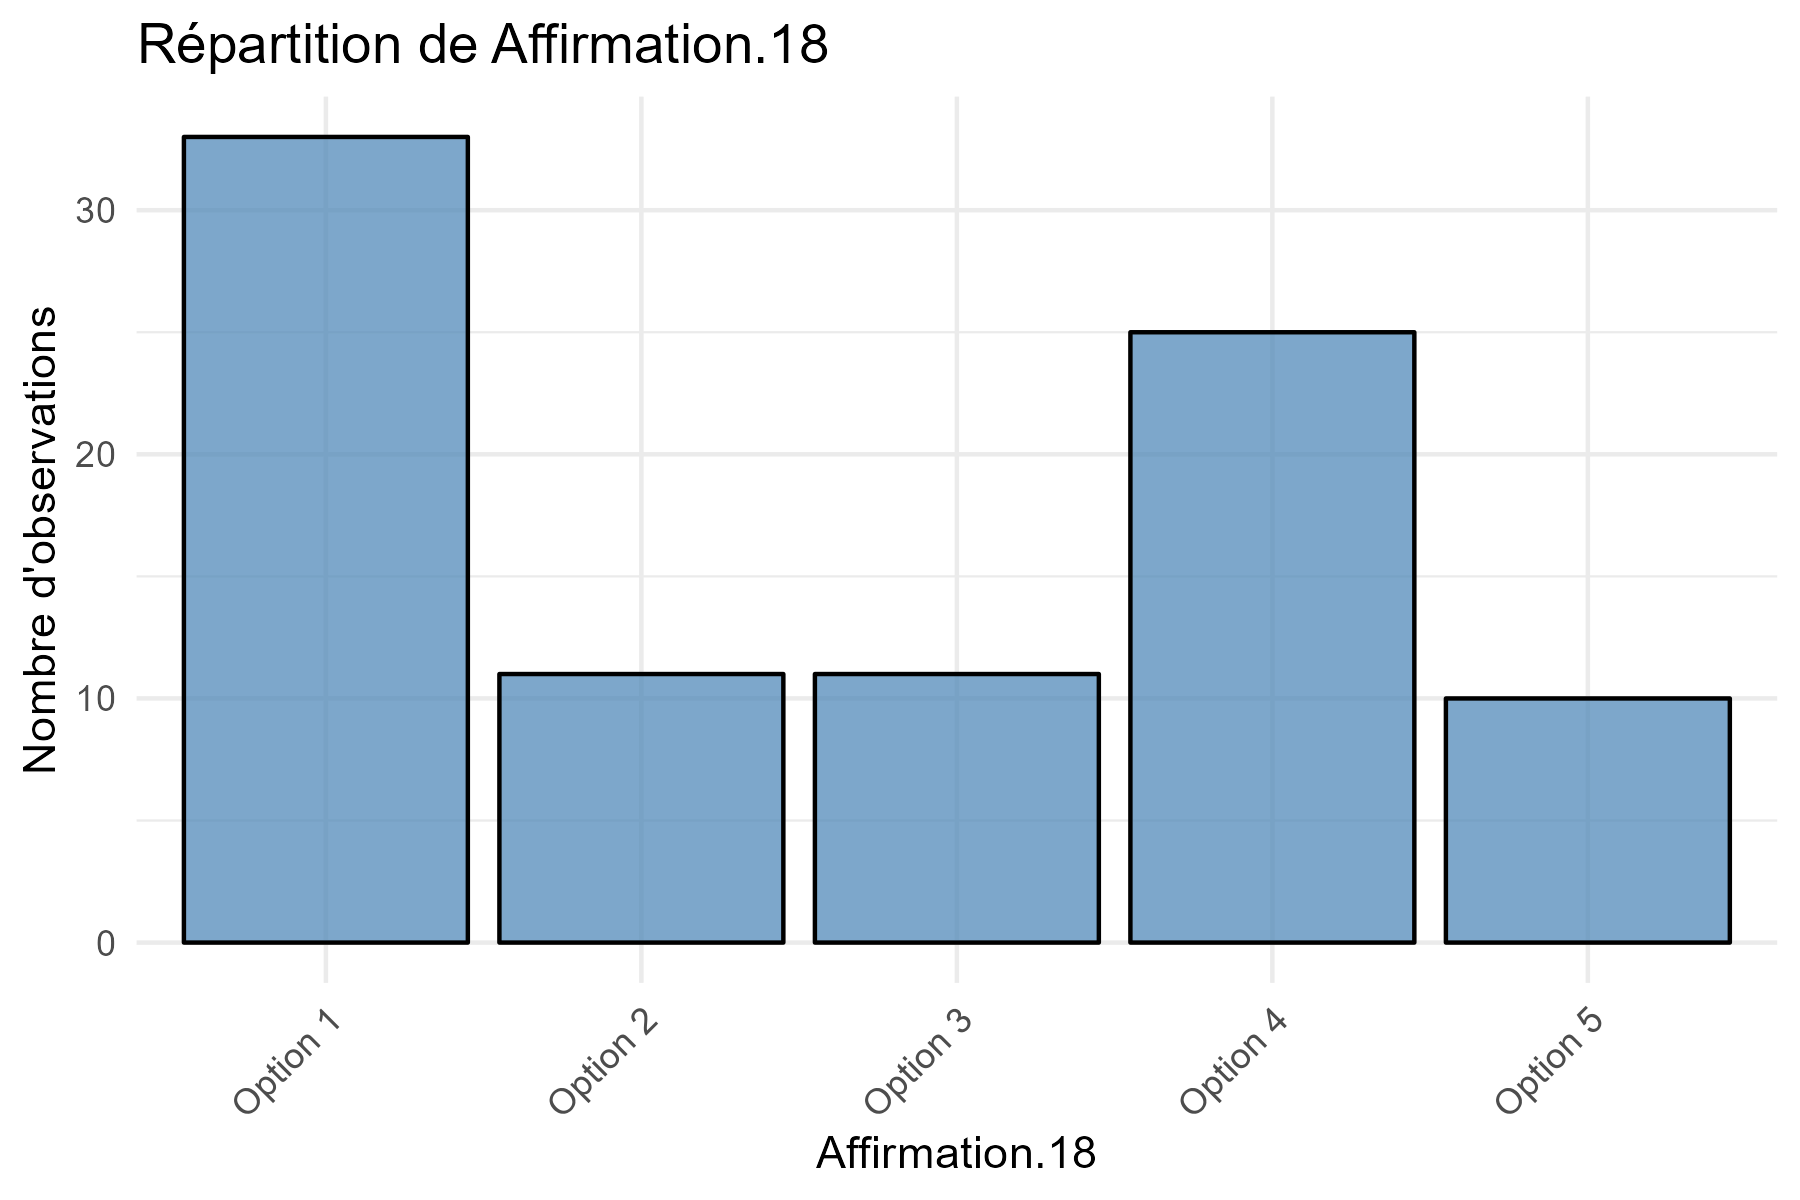
\includegraphics{Image/barplot_Affirmation.18.png}
\caption{barplot affirmation 18}
\end{figure}

\section{affirmation 19}\label{affirmation-19}

affirmation 19

\begin{figure}
\centering
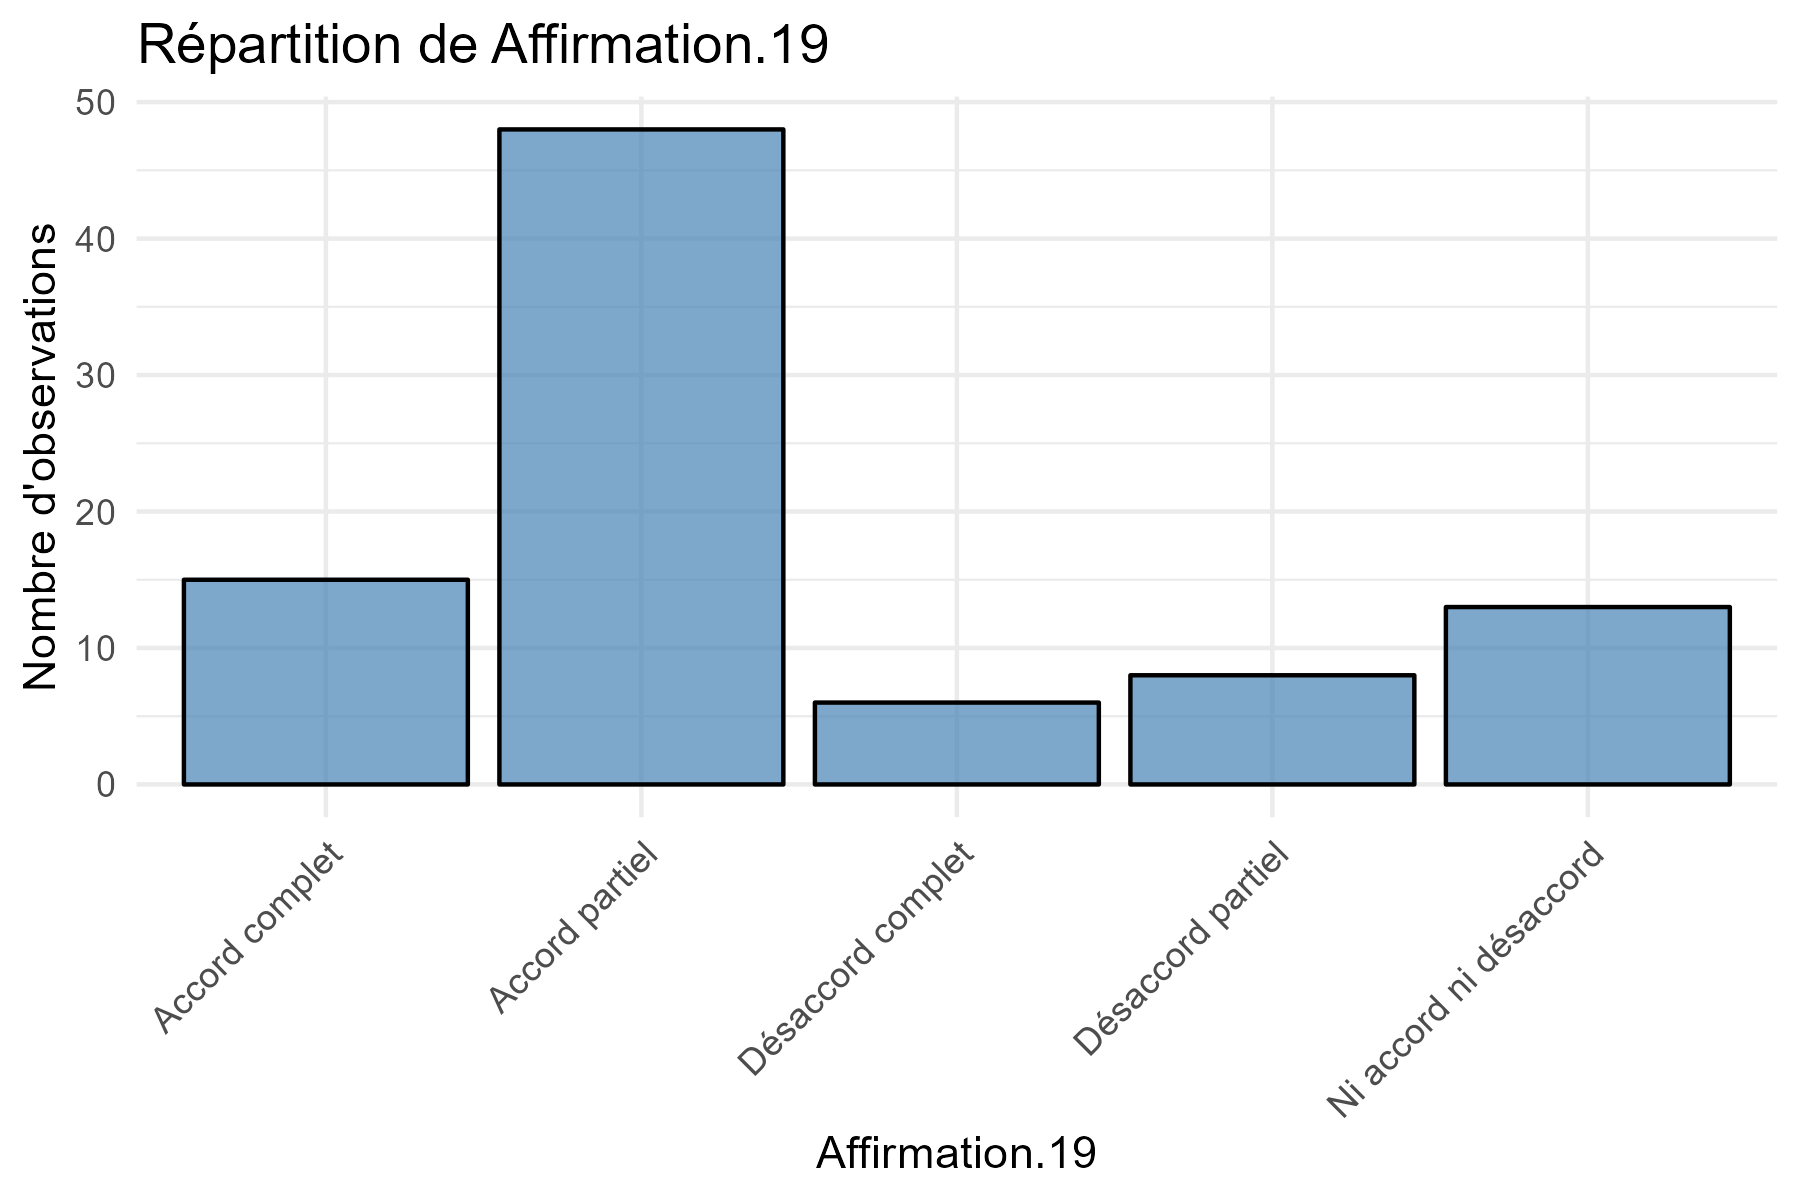
\includegraphics{Image/barplot_Affirmation.19.png}
\caption{barplot affirmation 19}
\end{figure}

\section{affirmation 110}\label{affirmation-110}

affirmation 110

\begin{figure}
\centering
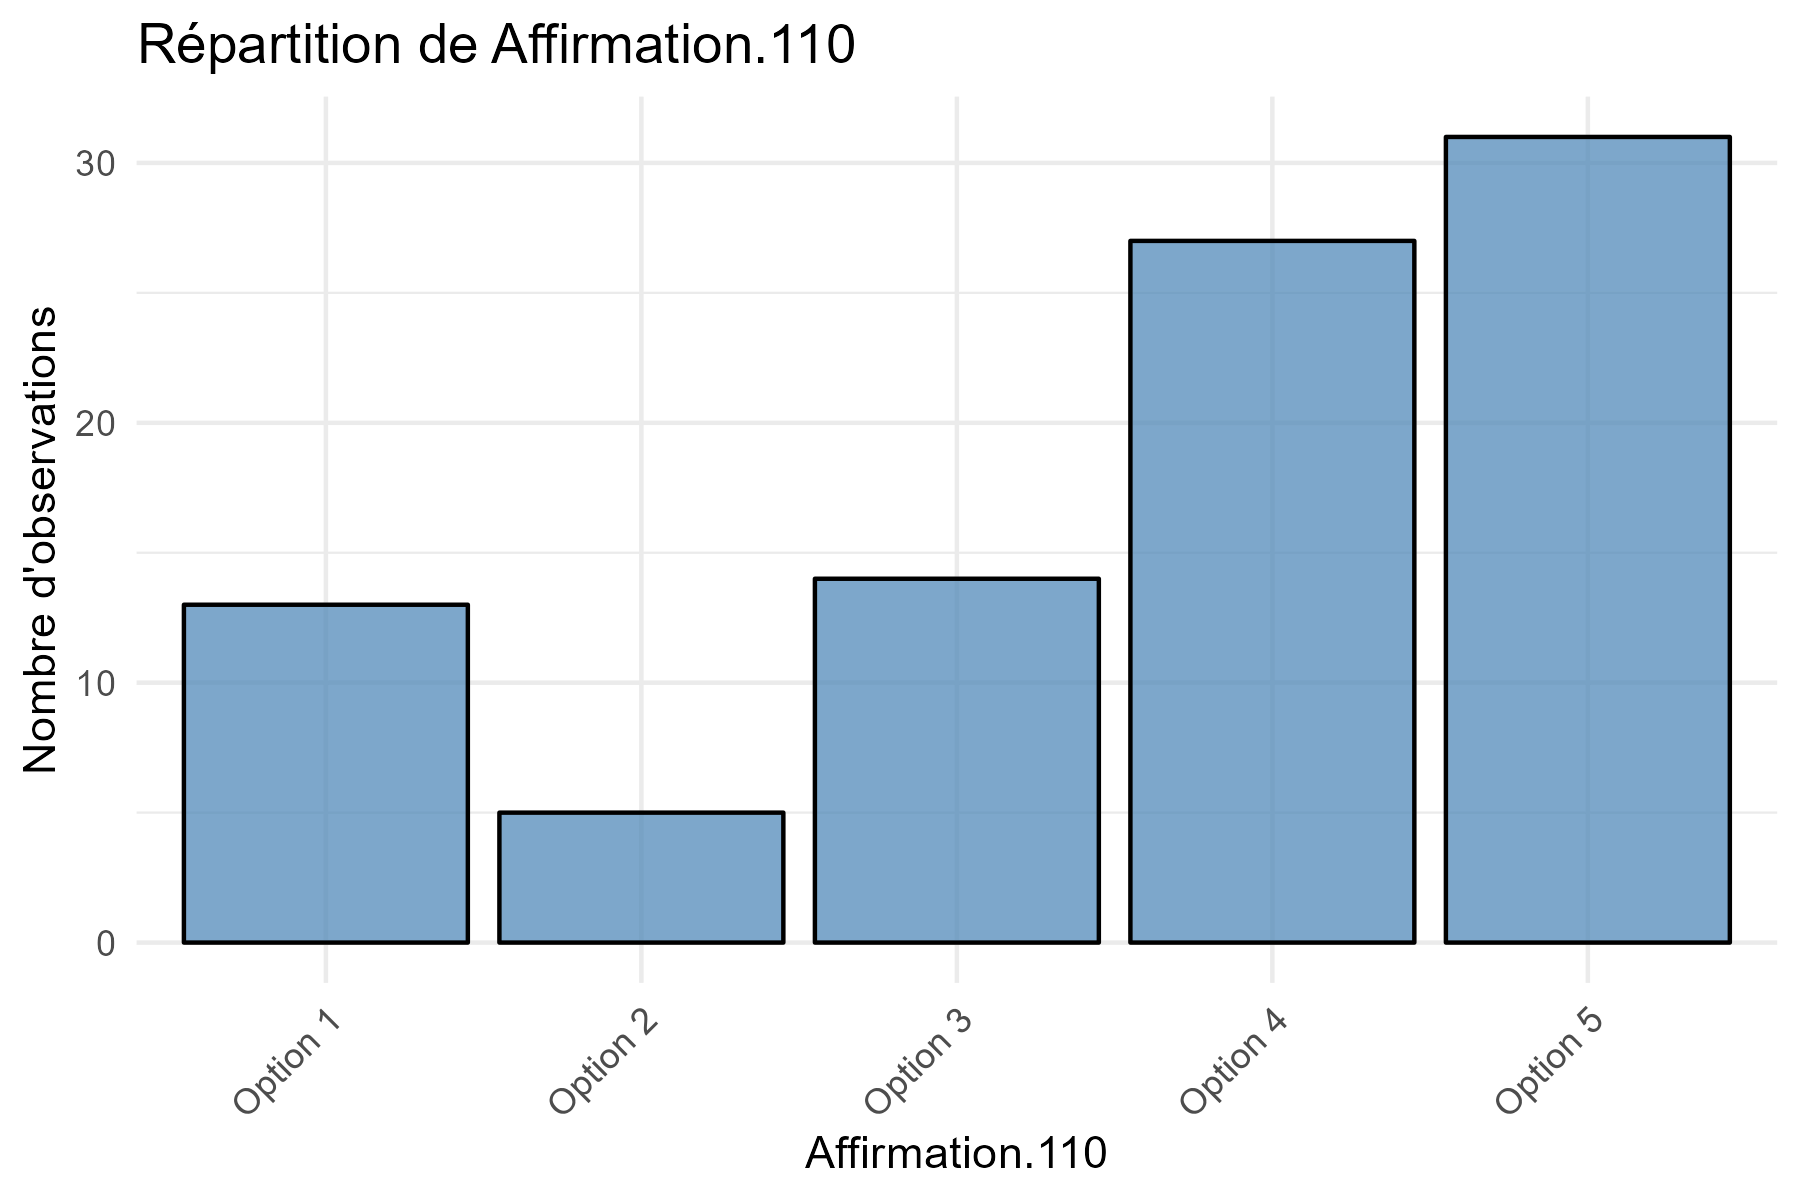
\includegraphics{Image/barplot_Affirmation.110.png}
\caption{barplot affirmation 110}
\end{figure}

\section{affirmation 111}\label{affirmation-111}

affirmation 111

\begin{figure}
\centering
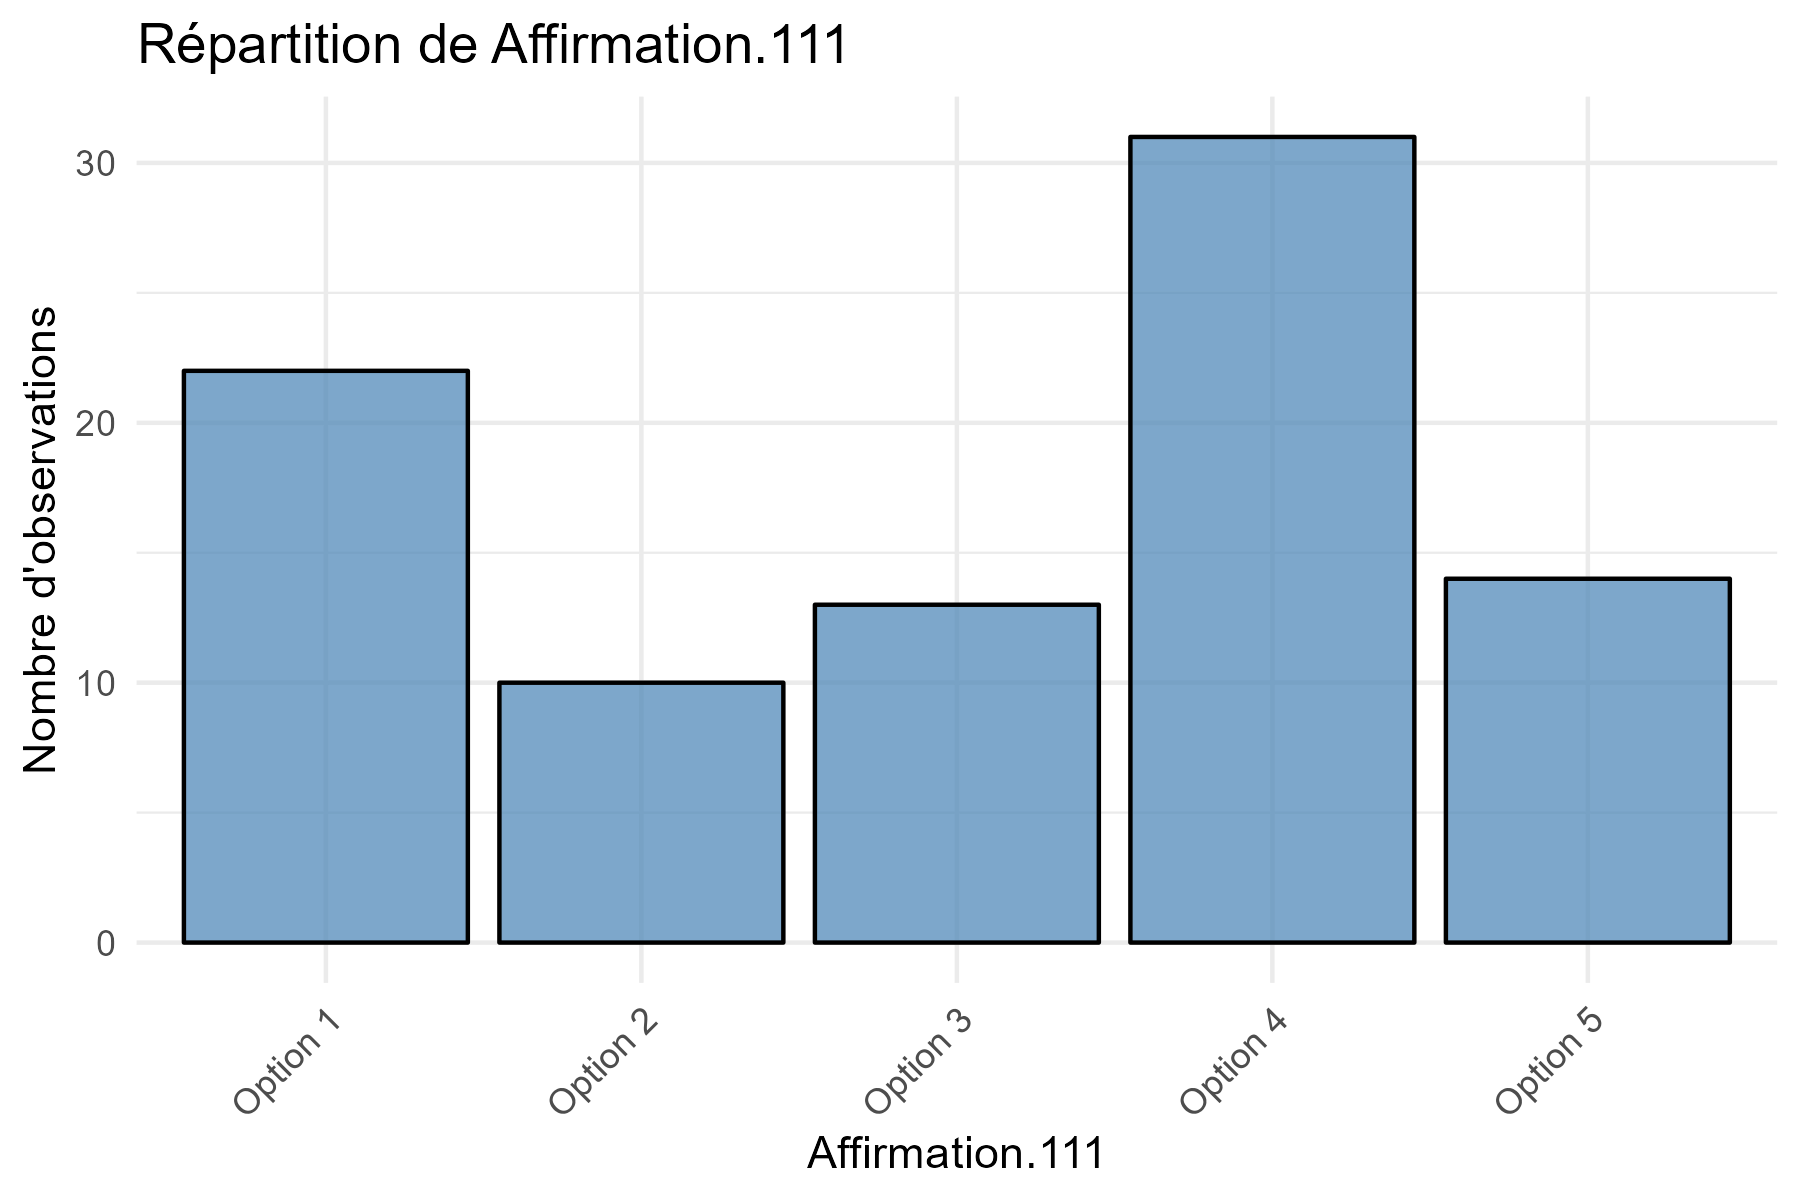
\includegraphics{Image/barplot_Affirmation.111.png}
\caption{barplot affirmation 111}
\end{figure}

\section{affirmation 112}\label{affirmation-112}

affirmation 112

\begin{figure}
\centering
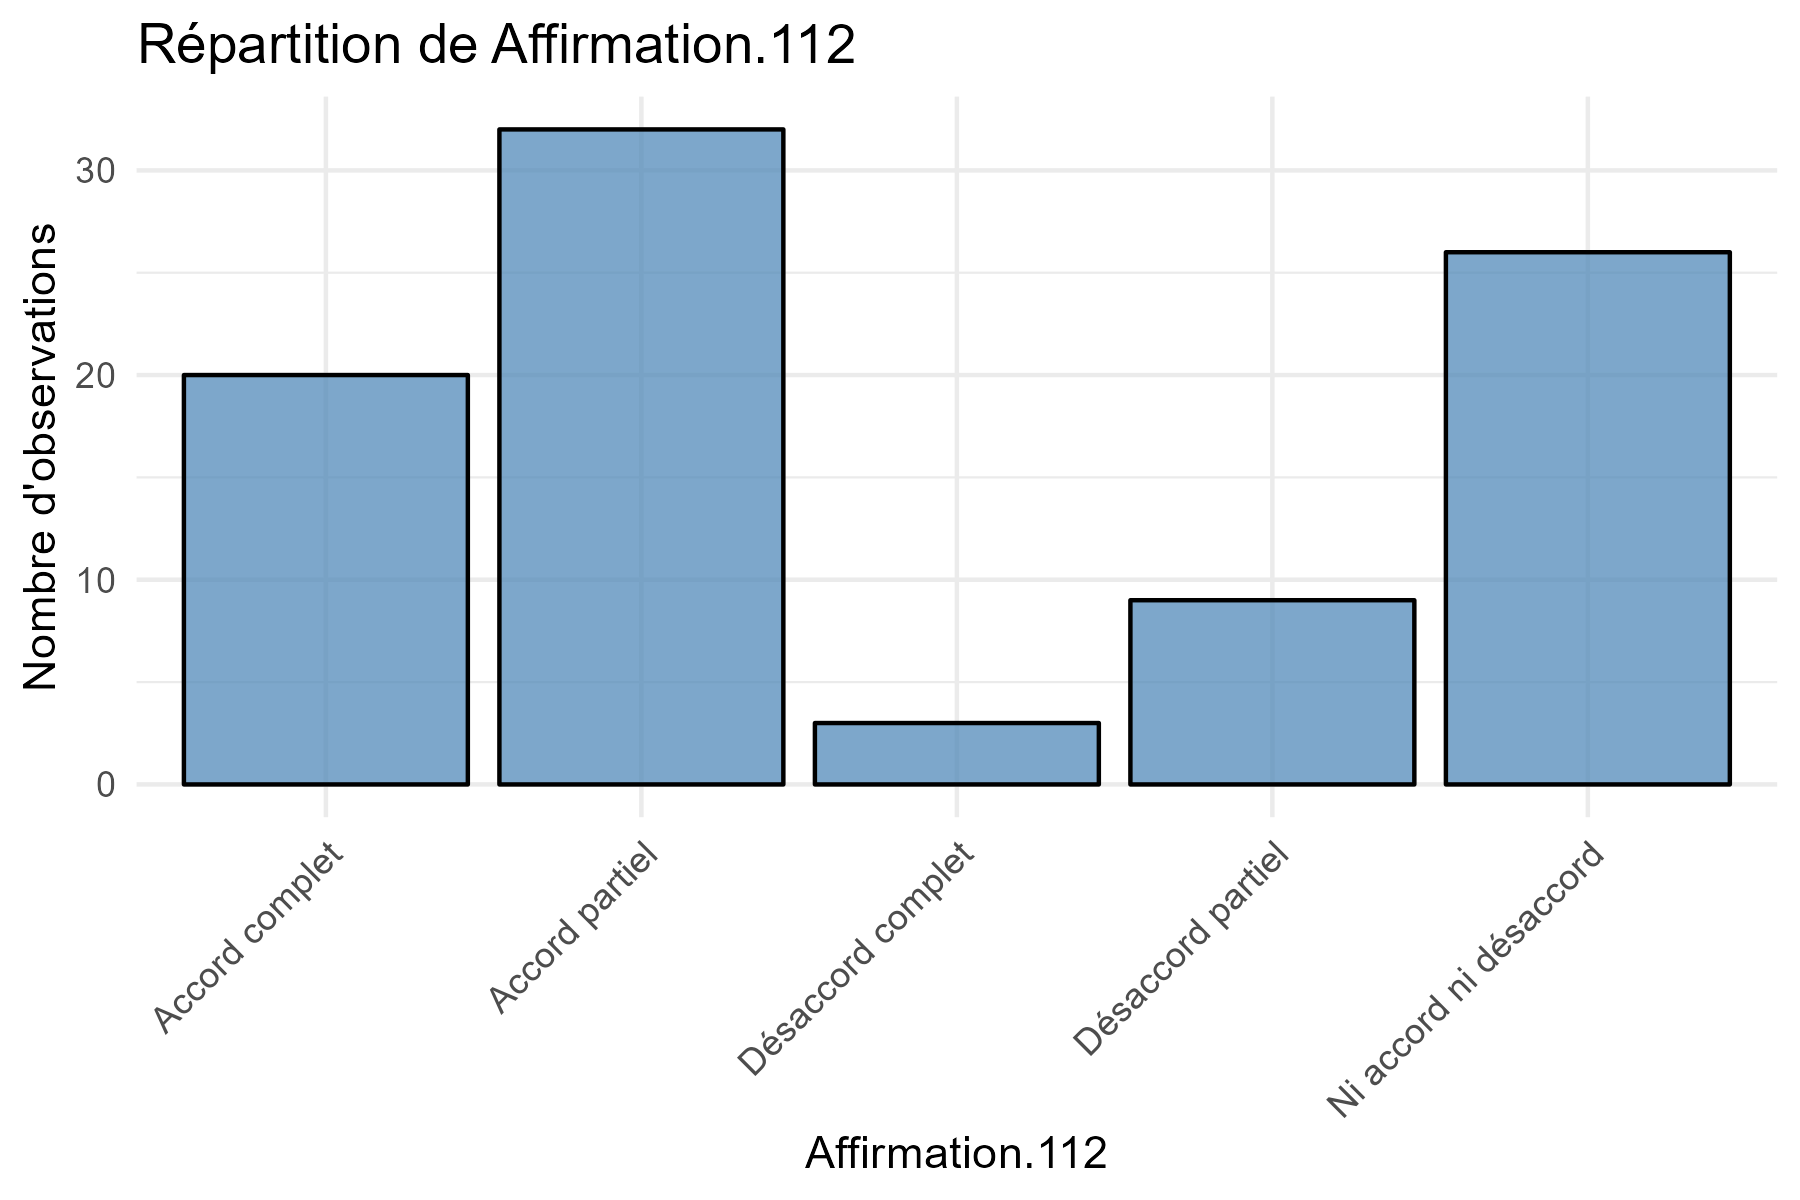
\includegraphics{Image/barplot_Affirmation.112.png}
\caption{barplot affirmation 112}
\end{figure}

\section{affirmation 113}\label{affirmation-113}

affirmation 113

\begin{figure}
\centering
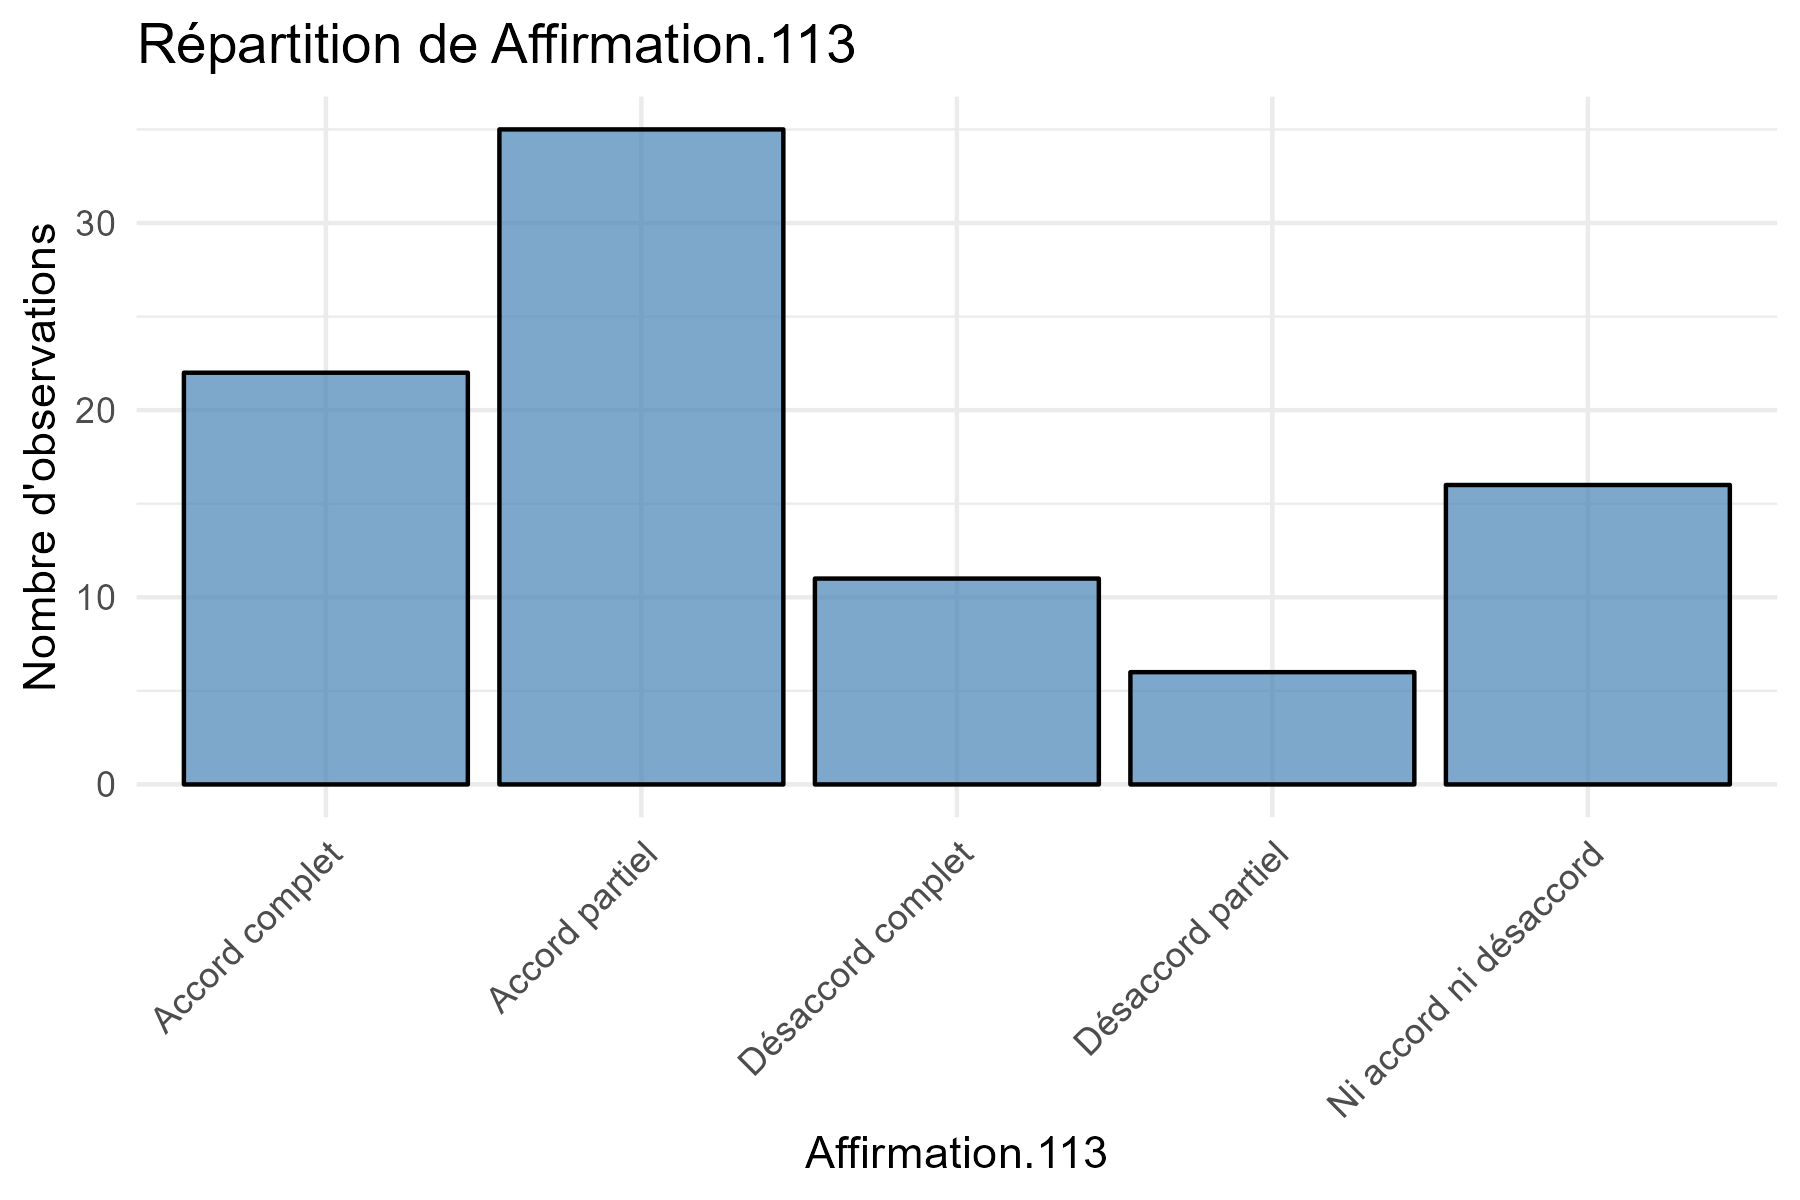
\includegraphics{Image/barplot_Affirmation.113.png}
\caption{barplot affirmation 113}
\end{figure}

\section{affirmation 114}\label{affirmation-114}

affirmation 114

\begin{figure}
\centering
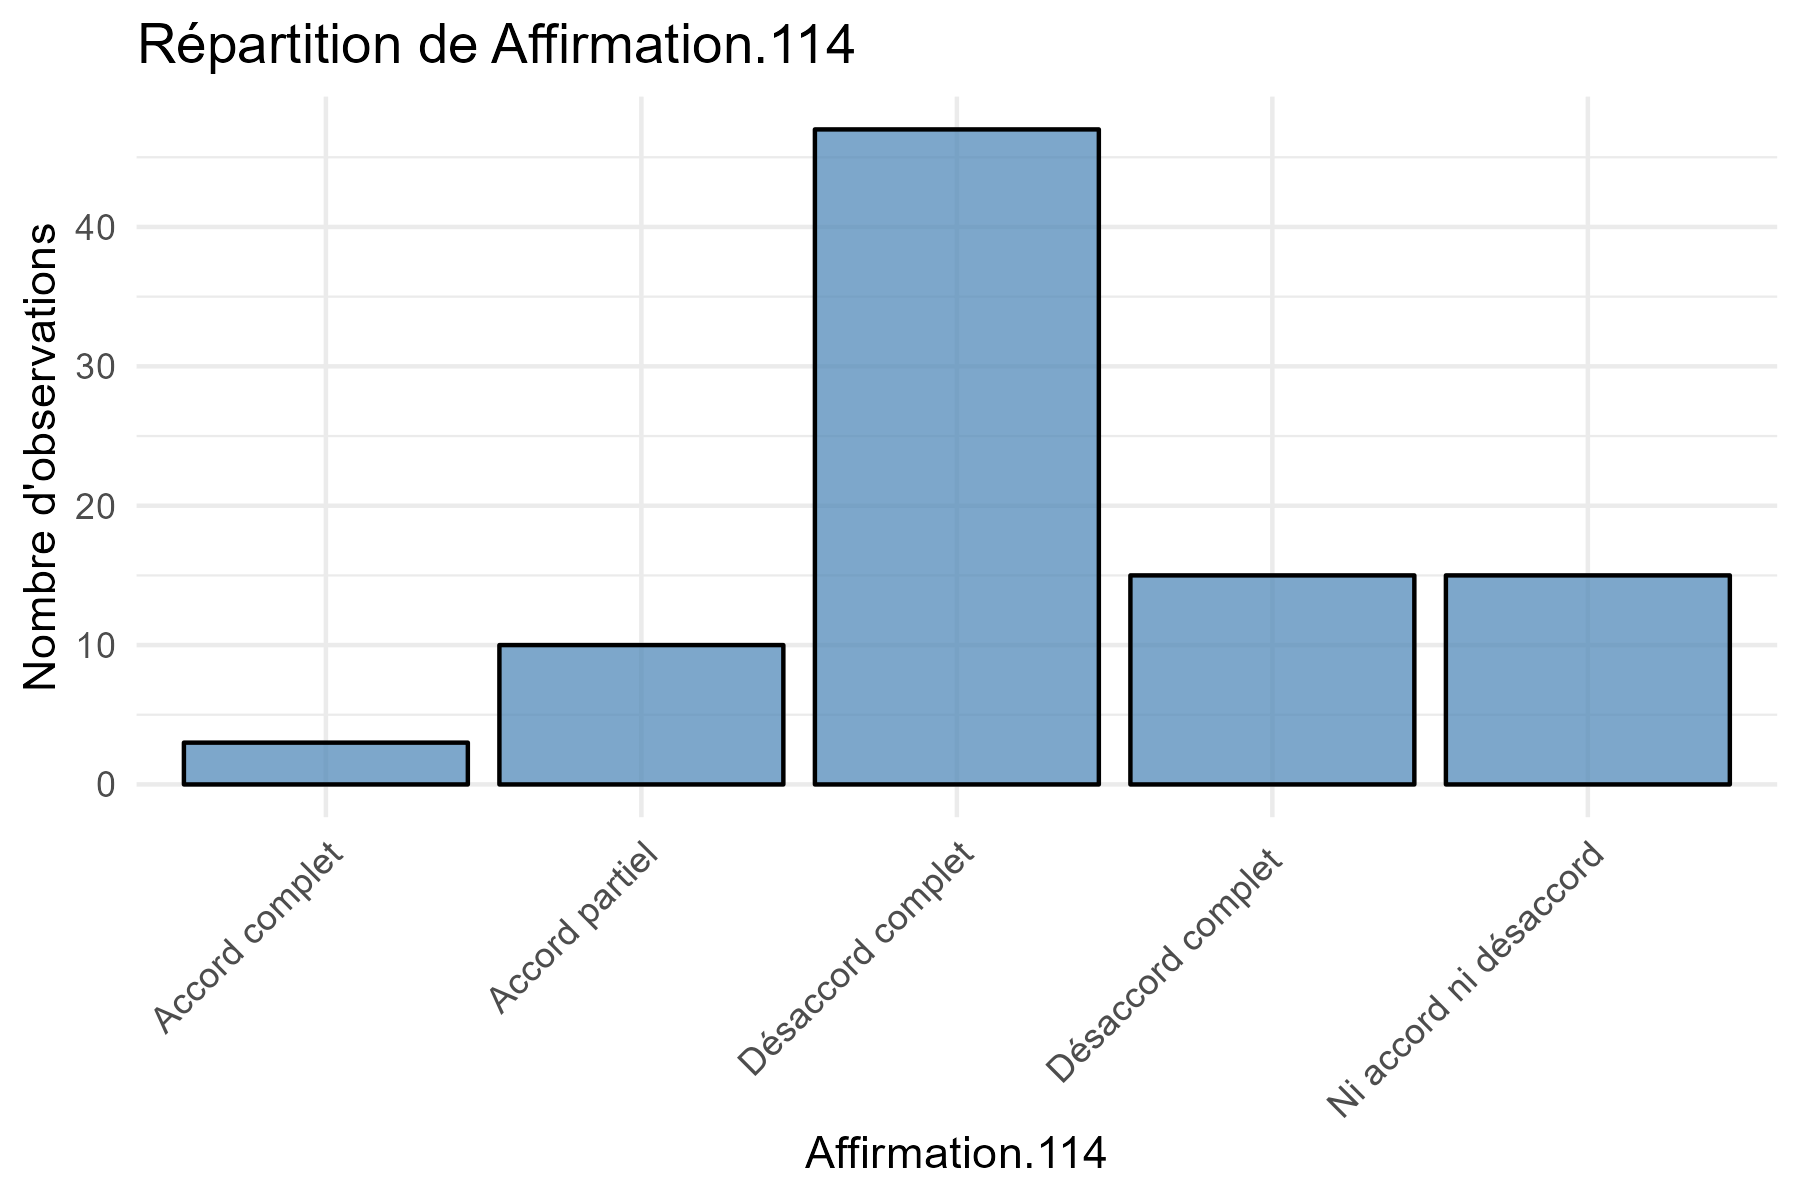
\includegraphics{Image/barplot_Affirmation.114.png}
\caption{barplot affirmation 114}
\end{figure}

\section{affirmation 115}\label{affirmation-115}

affirmation 115

\begin{figure}
\centering
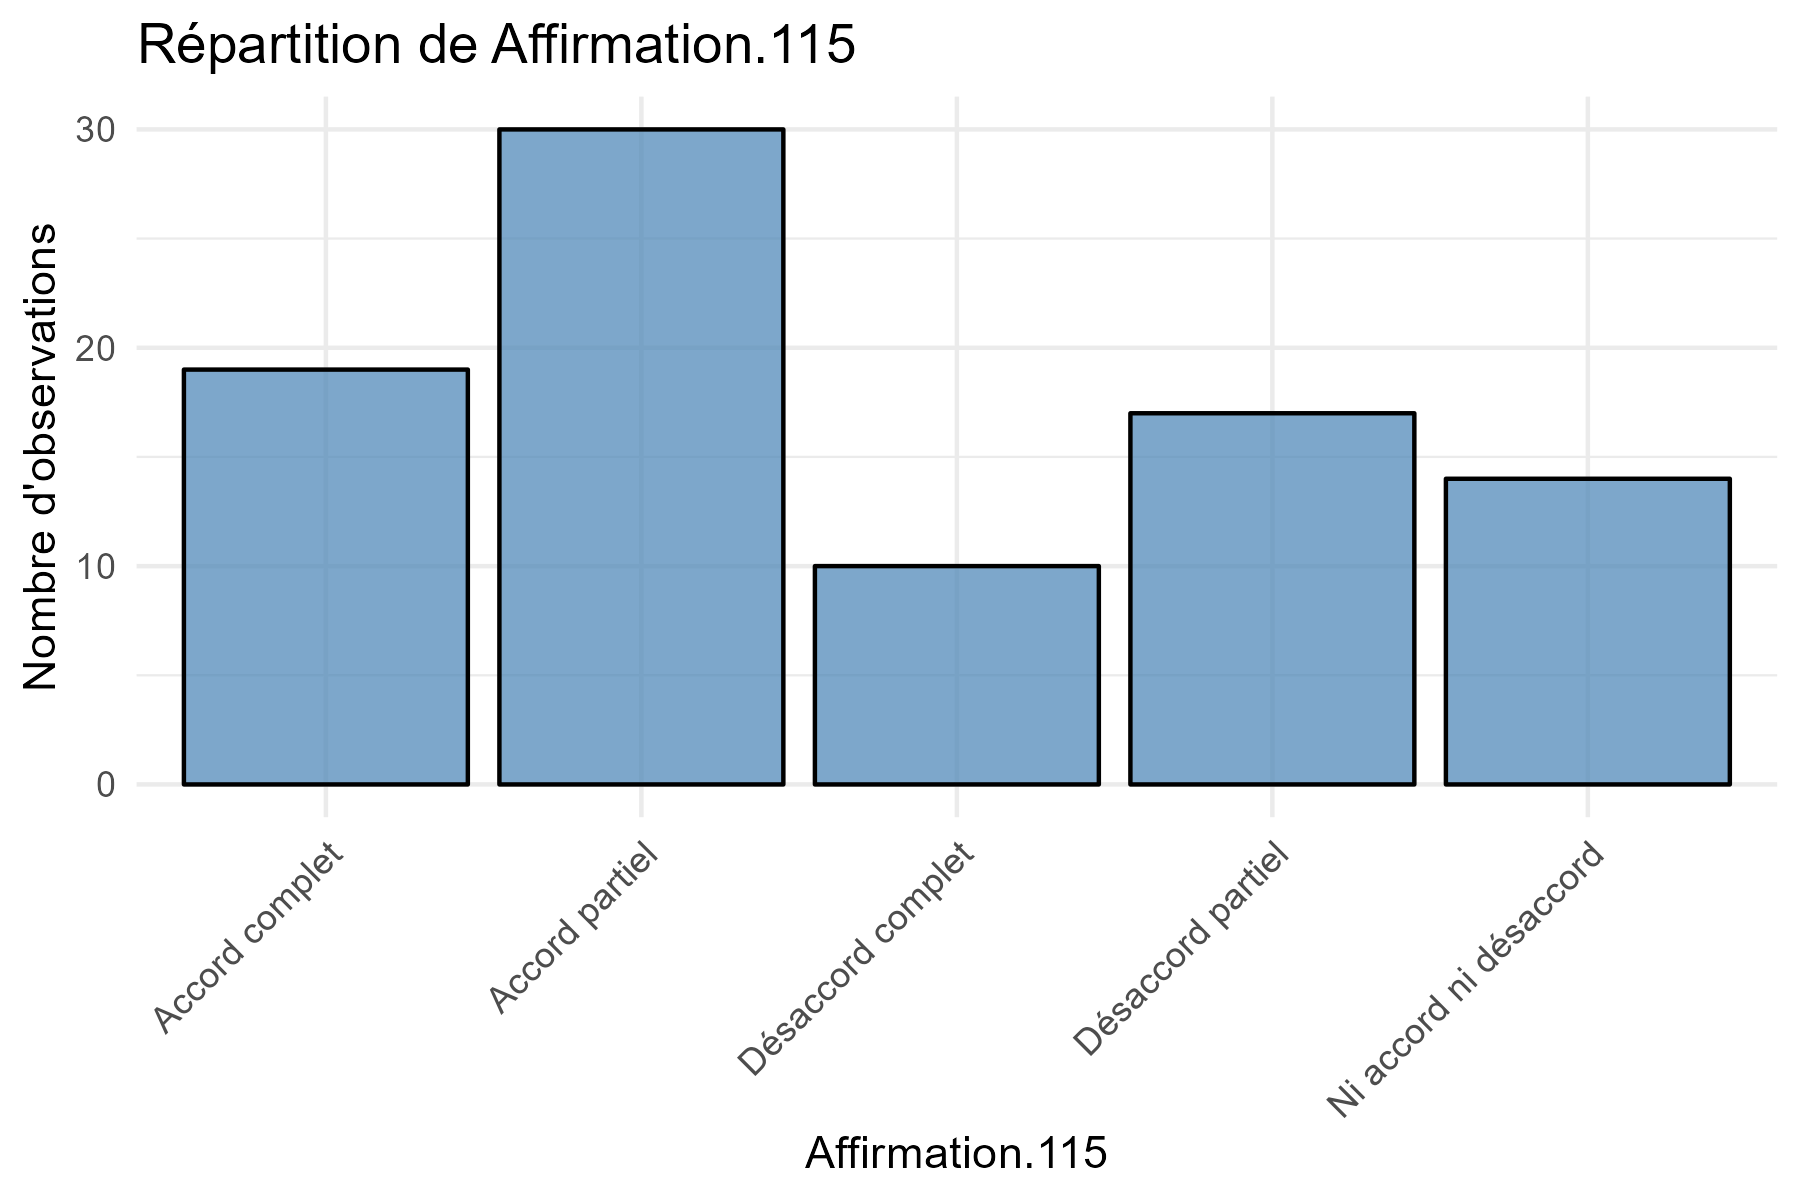
\includegraphics{Image/barplot_Affirmation.115.png}
\caption{barplot affirmation 115}
\end{figure}

\section{affirmation 116}\label{affirmation-116}

affirmation 116

\begin{figure}
\centering
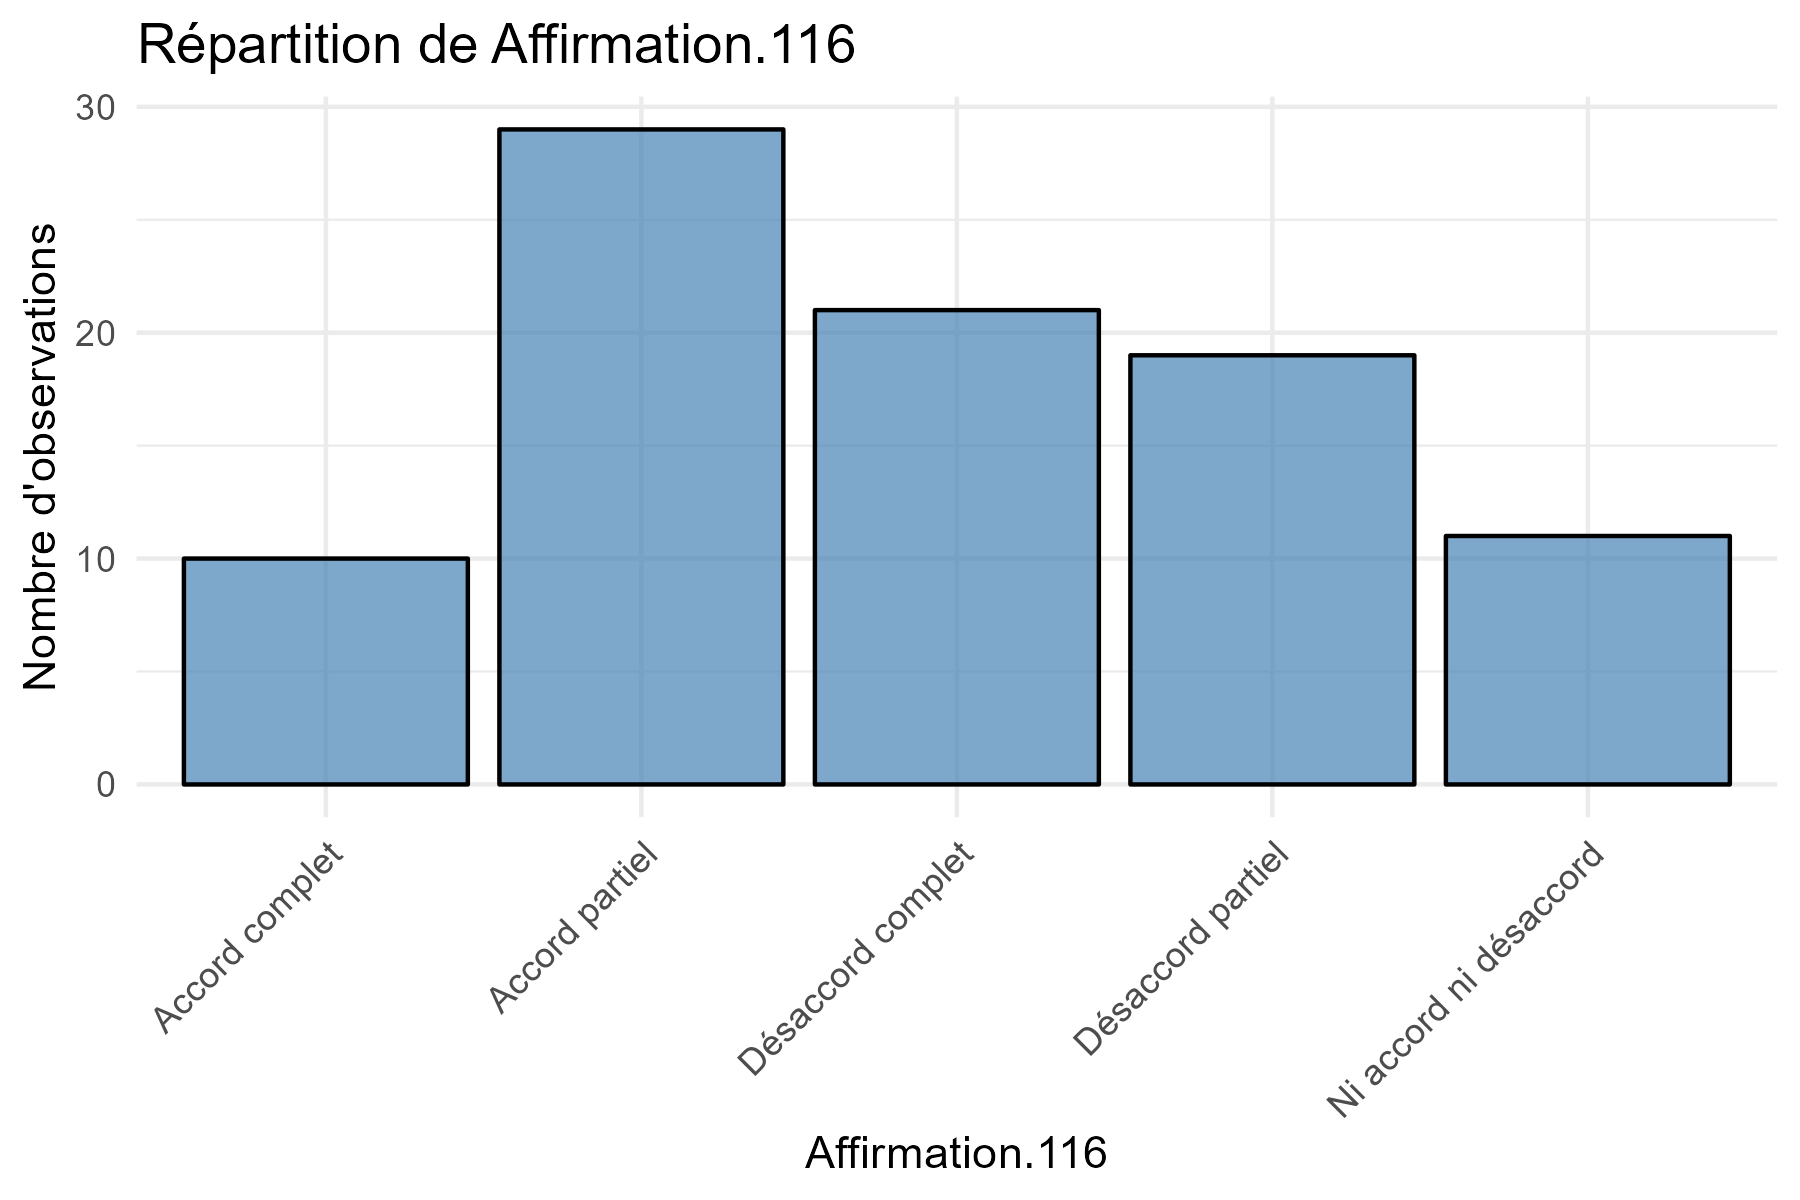
\includegraphics{Image/barplot_Affirmation.116.png}
\caption{barplot affirmation 116}
\end{figure}

\section{affirmation 117}\label{affirmation-117}

affirmation 117

\begin{figure}
\centering
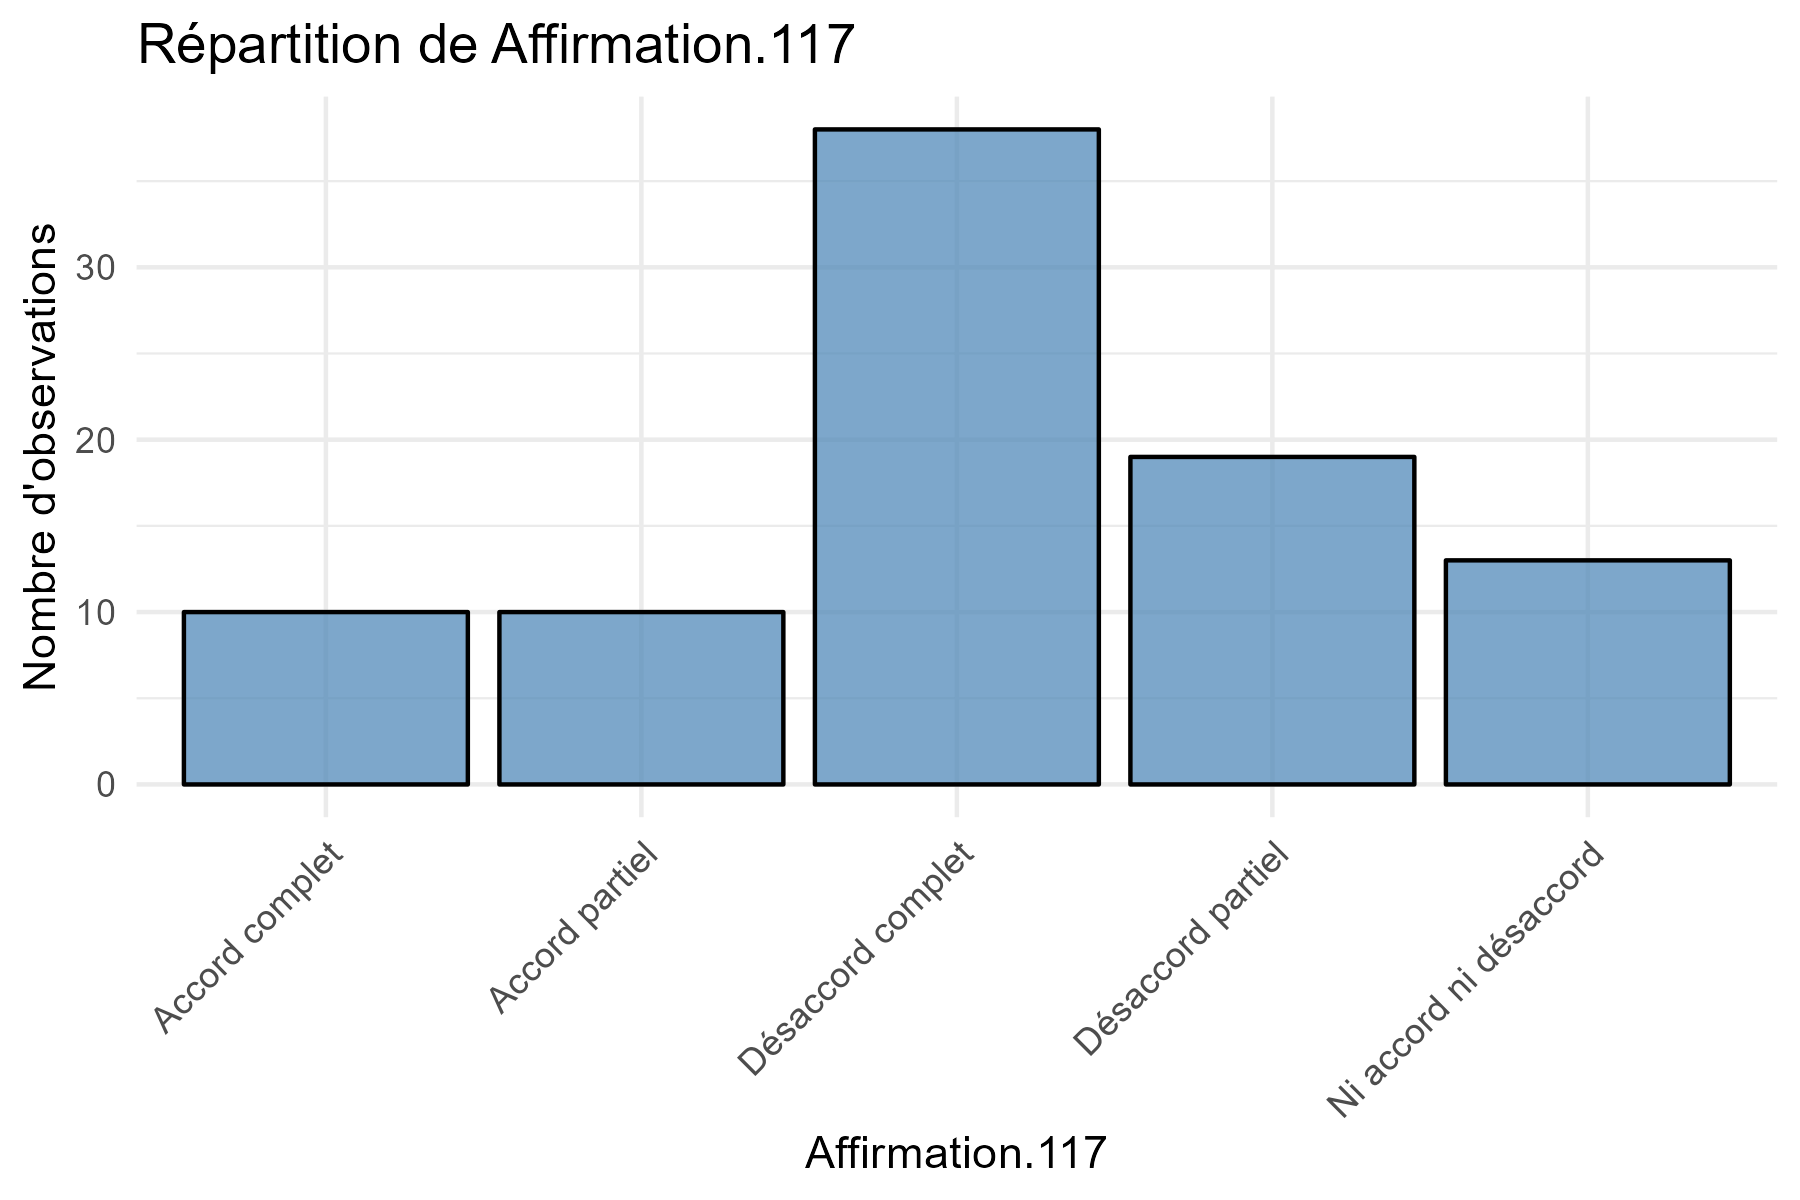
\includegraphics{Image/barplot_Affirmation.117.png}
\caption{barplot affirmation 117}
\end{figure}

\section{Conclusion}\label{conclusion}

Nos analyses montrent que les joueurs ayant plus d'expérience ont un
niveau d'anxiété globalement plus faible avant un match, bien que
certaines différences persistent selon le sexe. L'anxiété avant un match
est un facteur clé qui peut influencer la performance, et des stratégies
comme la préparation mentale ou la gestion du stress pourraient être
recommandées aux jeunes joueurs.

\subsubsection{``Limites de l'étude''}\label{limites-de-luxe9tude}

Cela rendra ton rapport plus rigoureux en précisant les éventuelles
faiblesses :

Échantillon limité 90 joureur. Données déclaratives (les joueurs peuvent
sous-estimer ou surestimer leur anxiété). Autres facteurs non étudiés
(fatigue, conditions climatiques\ldots).

\end{document}
